\documentclass{cubeamer}
\usepackage[style=authoryear, backend=biber, citetracker]{biblatex}
\usepackage{svg}
% \usepackage{showframe}
\usepackage{layout}
\usepackage{bm}
\usepackage{commath}
\usefonttheme{professionalfonts}
\usepackage{newpxmath}
\usepackage{siunitx}

\title{Accelerating Implicit Contact via Matrix-Free Operators on Non-Conforming Interfaces}
\subtitle[41st CCIMM]{41st Colorado Conference on Iterative and Multigrid Methods}
\author[Zachary R. Atkins]{\textbf{Zachary R. Atkins}\qquad\small Collaborators: Jed Brown and Jeremy L. Thompson}
\date{24 June 2026} % or whatever the date you are presenting in is
\institute[CU Boulder]{University of Colorado Boulder\\Department of Computer Science}

\setlength{\leftmargini}{0cm}
\setlength{\leftmarginii}{0.5cm}

\newlength{\textheightwithtitle}
\setlength{\textheightwithtitle}{6.6cm}
\newlength{\colratioone}
\newlength{\colratiotwo}

\newenvironment{twocolimgleft}[2][width=\textwidth,height=\textheightwithtitle]
{\begin{columns}
    \begin{column}{0.5\textwidth}
         \includesvg[#1]{#2}
     \end{column}
    \begin{column}{0.5\textwidth}
    }
    {
    \end{column}
\end{columns}}

\newenvironment{twocolimgleftratio}[3][width=\textwidth,height=\textheightwithtitle]
{\setlength{\colratioone}{\dimeval{\fpeval{#3*\textwidth}pt}}
\setlength{\colratiotwo}{\dimeval{\fpeval{\fpeval{1.0-#3}*\textwidth}pt}}
\begin{columns}
    \begin{column}{\colratioone}
        \includesvg[#1]{#2}
     \end{column}
    \begin{column}{\colratiotwo}
    }
    {
    \end{column}
\end{columns}}

\newcommand{\coverflag}{<+->}
% \renewcommand{\coverflag}{}

% Define a custom environment that forces early expansion
\newenvironment{flagitemize}
  {\expandafter\itemize\expandafter[\coverflag]}
  {\enditemize}

\newenvironment{flagenumerate}
  {\expandafter\enumerate\expandafter[\coverflag]}
  {\endenumerate}

% \setlength{\headheight}{1cm}
% \setlength{\textheight}{7cm}
% \setlength{\footskip}{0cm}
\setlength{\marginparsep}{0cm}
\setlength{\marginparwidth}{0cm}

\makeatletter
\define@key{beamerframe}{c}[true]{% centered
 \beamer@frametopskip=0pt plus 1fill\relax%
 \beamer@framebottomskip=0pt plus 1fill\relax%
 \beamer@frametopskipautobreak=0pt plus .4\paperheight\relax%
 \beamer@framebottomskipautobreak=0pt plus .6\paperheight\relax%
 \def\beamer@initfirstlineunskip{}%
}
\makeatother

\addbibresource{references.bib}
\setbeamerfont{footnote}{size=\tiny} %reduce the size of the footnote citation
\setbeamerfont{bibliography item}{size=\scriptsize}
\setbeamerfont{bibliography entry author}{size=\scriptsize}
\setbeamerfont{bibliography entry title}{size=\scriptsize}
\setbeamerfont{bibliography entry location}{size=\scriptsize}
\setbeamerfont{bibliography entry note}{size=\scriptsize}
\renewcommand*{\bibfont}{\tiny}

\newcommand{\abr}[1]{\left\langle {#1} \right\rangle}

\begin{document}

\maketitle

\begin{frame}{Outline}
    \tableofcontents
\end{frame}

\begin{frame}{Acknowledgments}
\small
This work was supported by the Department of Energy, National Nuclear Security Administration, \alert{Predictive Science Academic Alliance Program (PSAAP III)} under Award Number DE-NA0003962, and by the Department of Energy Frameworks, Algorithms, and Scalable Technologies for Mathematics (FASTMath) \alert{SciDAC Institute} and the U.S. Department of Energy, Office of Science, Office of Advanced Scientific Computing Research under contract DE-AC02-05CH11231 and Award Number DE-SC0016140.
\end{frame}

\section{General Matrix-Free FEM}

\begin{frame}{libCEED Matrix-Free Formulation}
    \centering
    \includesvg[height=0.65\textheightwithtitle]{img/libCEED-decomposition}
    \vspace{-0.05\textheightwithtitle}
\only<2>{\begin{alertblock}{Partitioning}
    The operator $\mathcal P$ represents mapping from the parallel vector to the local vector, including inserting ghost values --- this is done using PETSc's \texttt{DMPlex}
\end{alertblock}}
\only<3>{\begin{alertblock}{Element Restriction}
    The operator $\mathcal E$ maps local degrees-of-freedom to the finite element vector via duplicating values at nodes shared between elements
\end{alertblock}}
\only<4>{\begin{alertblock}{Basis}
    The operator $B$ represents interpolation and/or gradient from nodes to quadrature points
\end{alertblock}}
\only<5>{\begin{alertblock}{Quadrature Function}
    The operator $D$ represents the action of the PDE \& its linearization at individual quadrature points --- this is where all of the physics is defined
\end{alertblock}}
\end{frame}


\begin{frame}{Matrix-Free FEM}
\begin{block}{Generic Weak Form}
    Find $\bm u\in \mathcal{V}\subset H^1(\Omega)$ such that for all $\bm v \in\mathcal{V}$,
    \begin{equation*}
        \abr{\bm v, \bm u} = \int_{\Omega} \sbr{\bm v \cdot f_0 \del{\bm u, \nabla \bm u} + \nabla \bm v : f_1\del{\bm u, \nabla \bm u}} \dif V + \int_{\partial \Omega} \bm v \cdot g_{0} \del{\bm u, \nabla \bm u} \dif A = 0,
    \end{equation*}
\end{block}
\uncover<2->{\begin{alertblock}{Tensor Product Assumptions}
    We will assume that $\mathcal{V}$ is a sum-factorizable finite element space defined over tensor product elements.
\end{alertblock}}
\end{frame}

\section{Numerical Contact Evaluation}

\begin{frame}{Model Problem}
\begin{columns}
    \begin{column}{0.5\textwidth}
        Consider two elastic bodies $\Omega_1, \Omega_2$.
        
        In the following,
        \begin{align*}
            f_0(\bm u, \nabla \bm u) &= \bm 0, f_1(\bm u, \nabla \bm u) = \bm P(\nabla \bm u)\\
            g_0(\bm u, \nabla \bm u) &= \lambda_n(u) \text{ (contact forces)}\\
            &= -\sbr{\epsilon g(\bm u)}_{\mathbb{R}^-} \bm{n}_x
        \end{align*}
        In general, KKT conditions:
        \[
        g(u) \geq 0,\quad \lambda_n(u) \geq 0, \quad g(u) \cdot \lambda_n(u) = 0. 
        \]
        Need to \alert{integrate} gap function $g(\bm u)$ over \alert{common contact surface}
    \end{column}
    \begin{column}{0.5\textwidth}
        \centering
        \includesvg[width=\textwidth,height=\textheightwithtitle]{img/contact_hertz_fbd_full}
    \end{column}
\end{columns}
\end{frame}

\begin{frame}{Discretized Model Problem}
\centering
\only<1>{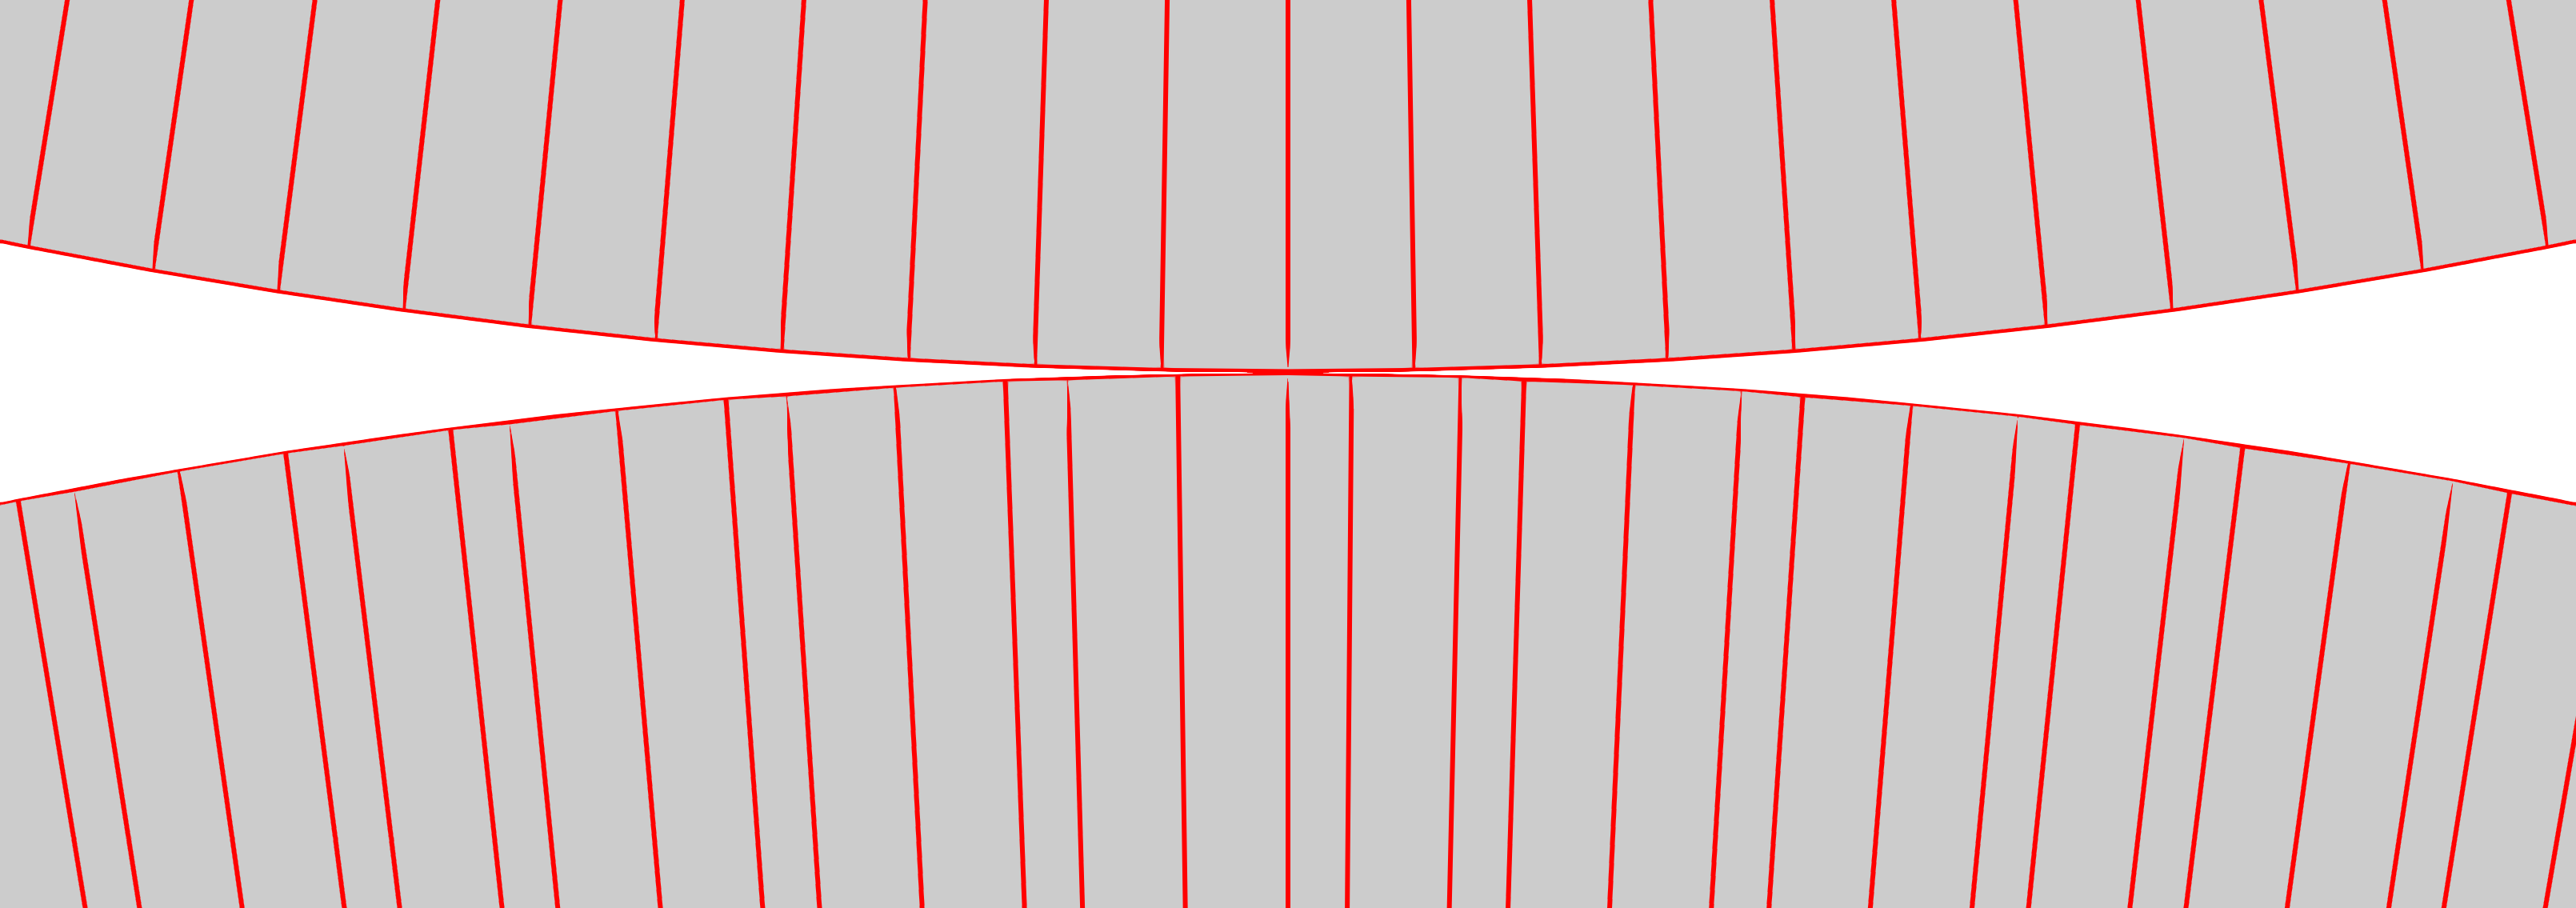
\includegraphics[height=0.6\textheightwithtitle]{img/non-matching-mesh-cropped.png}}
\only<2>{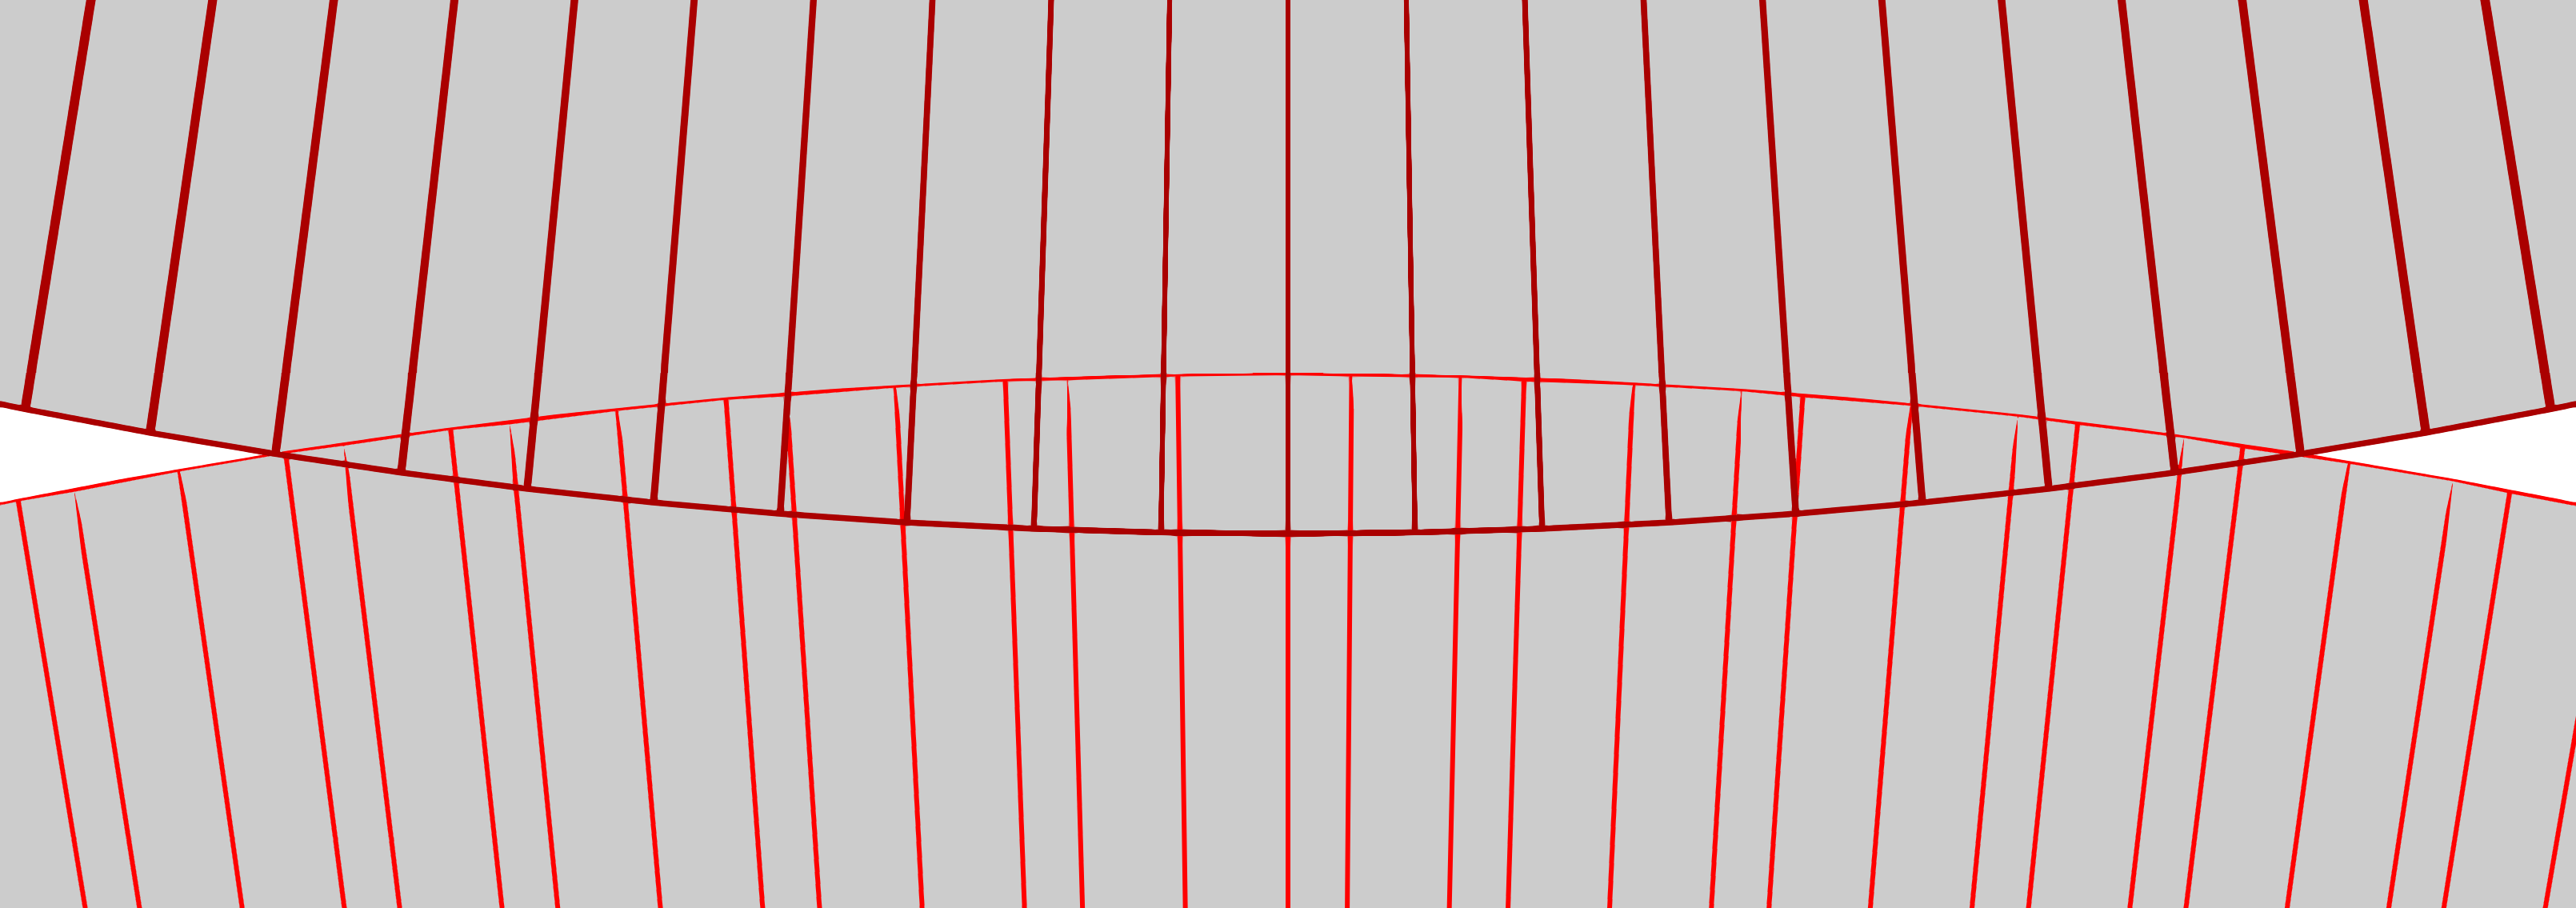
\includegraphics[height=0.6\textheightwithtitle]{img/non-matching-mesh-overlap-cropped.png}}
\only<3>{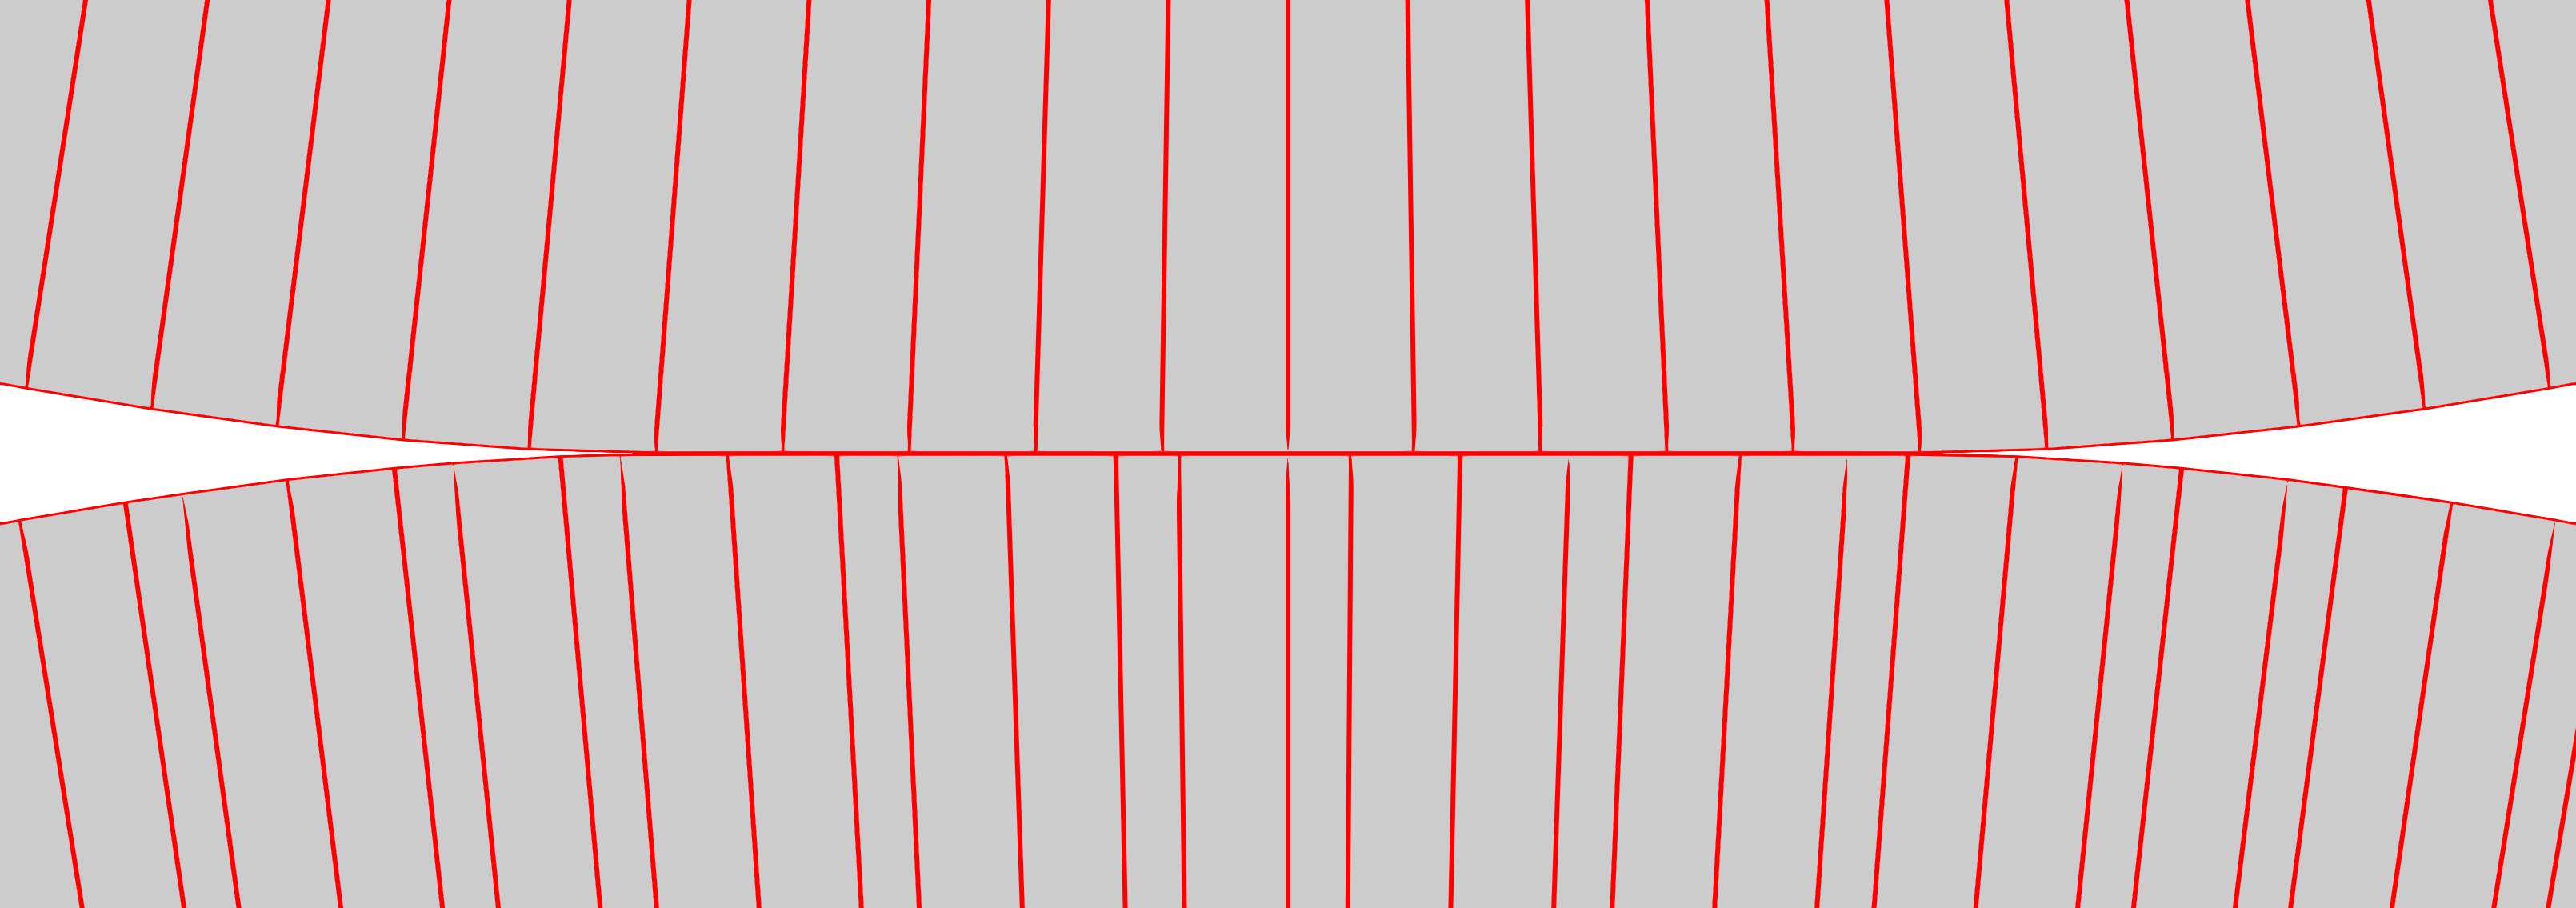
\includegraphics[height=0.6\textheightwithtitle]{img/non-matching-mesh-converged-cropped.png}}
\vspace{2em}
\begin{columns}
    \begin{column}{0.1\textwidth}\end{column}
    \begin{column}{0.8\textwidth}
    \centering
    \only<1>{In reality, bodies are represented as discrete meshes, usually with non-conforming/non-matching contact interfaces}
    \only<2>{When penetration occurs, it does so with arbitrary overlap between the face elements on either side}
    \only<3>{Ultimately, need to find displacements $\bm u^h$ such that the discrete gap $g(\bm u^h) \to 0$ in a weak sense along the contact interface}
    \end{column}
    \begin{column}{0.1\textwidth}\end{column}
\end{columns}

\end{frame}

\subsection{Mortar Method for Segmentation-Based Contact}
\begin{frame}{Simple Case: Two Linear Quadrilateral Facets}
\begin{twocolimgleft}{img/segmentation_step_01.svg}
    \begin{flagitemize}
        \item Clearly, these facets overlap, but they are not in the same plane
        \begin{itemize}
            \item Formally, their intersection is a segment
        \end{itemize}
        \item Goal: define some non-zero area where the facets are in contact
    \end{flagitemize}
\end{twocolimgleft}
\end{frame}

\begin{frame}{Mortar Method for Segmentation-Based Contact}
\begin{twocolimgleft}{img/segmentation_step_01.svg}
    \begin{flagitemize}
        \item Consider a well established approach from \cite{Puso_Laursen_2004}
        \item Label one face as the "non-mortar" face, where integration will be well defined
        \item Label the other face as the "mortar" face, which will experience some aliasing during integration
        \item We briefly outline the method (performed once per face pair per residual evaluation)
    \end{flagitemize}
\end{twocolimgleft}
\end{frame}

\begin{frame}{Project Mortar to Non-Mortar}
\begin{twocolimgleft}{img/segmentation_step_02.svg}
    \begin{flagitemize}
        \item Project the vertices of the other face onto the common plane of the non-mortar face
        \begin{itemize}
            \item If the non-mortar face vertices are not coplanar, use the midpoint and average face normal
        \end{itemize}
        \item The mortar face will experience some aliasing during integration due to the projection
    \end{flagitemize}
\end{twocolimgleft}
\end{frame}

\begin{frame}{Clip the 2D Polygons}
\begin{twocolimgleft}{img/segmentation_step_03.svg}
    \begin{flagitemize}
        \item Coplanar facets $\implies$ can directly find their intersection
        \item Very difficult to do robustly, especially for non-convex facets
        \item We use an algorithm by \cite{Greiner_Hormann_1998} with robustness improvements by \cite{Foster_Hormann_Popa_2019}
    \end{flagitemize}
\end{twocolimgleft}
\end{frame}

\begin{frame}{Triangulate the Clipped Polygon}
\begin{twocolimgleft}{img/segmentation_step_04.svg}
    \begin{flagitemize}
        \item Partition the clipped element into triangles
        \begin{itemize}
            \item We use a deterministic linear-time ear cut method by \cite{Livesu_Cherchi_Scateni_Attene_2022}
        \end{itemize}
        \item Assign quadrature points to the triangles using your preferred method
        \begin{itemize}
            \item We use symmetric quadrature rules by \cite{JaskowiecSukumar2021}
        \end{itemize}
        \item Assign integration weights $w_i \det J$, where 
        \begin{itemize}
            \item $w_i$ is the quadrature weight
            \item $\det J = \frac{\partial \bm x}{\partial\xi_1} \times \frac{\partial \bm x}{\partial\xi_2}$ is the Jacobian of the reference element mapping
        \end{itemize}
    \end{flagitemize}
\end{twocolimgleft}
\end{frame}

\begin{frame}{Mapping Back to the Mortar Surface}
\setlength{\colratioone}{\dimeval{\fpeval{0.33*\textwidth}pt}}
\setlength{\colratiotwo}{\dimeval{\fpeval{\fpeval{1.0-0.33}*\textwidth}pt}}
\begin{columns}
    \begin{column}{\colratioone}
        \only<2>{\includesvg[width=\textwidth,height=\textheightwithtitle]{img/segmentation_step_05.1_mortar.svg}}
        \only<3>{\includesvg[width=\textwidth,height=\textheightwithtitle]{img/segmentation_step_05.2_mortar.svg}}
        \only<4->{\includesvg[width=\textwidth,height=\textheightwithtitle]{img/segmentation_step_05_mortar.svg}}
    \end{column}
    \begin{column}{\colratiotwo}
    \begin{flagitemize}
        \item Reverse the projection for point $p$:
        \begin{flagenumerate}
            \item \alert{Ref-to-real}: interpolate $\bm{\xi}_p^{\textrm{tri}}\mapsto \bm{x}_p^{\textrm{proj}}$ with triangle geometry
            \item \alert{Real-to-ref}: $\bm{x}_p^{\textrm{proj}}\mapsto \bm{\xi}_p^{\textrm{mortar}}$ via local Newton solve with \textbf{projected} mortar nodal coordinates and Jacobian
            \item \alert{Ref-to-real}: interpolate $\bm{\xi}_p^{\textrm{mortar}}\mapsto\bm{x}_p^{\textrm{real, mortar}}$ with the \textbf{true} mortar facet geometry
        \end{flagenumerate}
        \item That is, the reference coordinates for each point with respect to the mortar face are computed in the projected space, then remain constant
    \end{flagitemize}
    \end{column}
\end{columns}
\end{frame}


\begin{frame}{Resulting Points on Each Side}
\begin{columns}
    \begin{column}{0.5\textwidth}
         \begin{figure}
             \centering
             \includesvg[scale=0.35]{img/segmentation_step_06_mortar.svg}
         \end{figure}
    \end{column}
    \begin{column}{0.5\textwidth}
        \begin{figure}
             \centering
             \includesvg[scale=0.35]{img/segmentation_step_06_nonmortar.svg}
         \end{figure}
    \end{column}
\end{columns}
\centering
Each side has the same points, just with different coordinates!
\end{frame}

\begin{frame}{Computing the Integral Over the Surface}
\begin{twocolimgleftratio}{img/segmentation_multi.svg}{0.5}
    \begin{flagitemize}
        \item Repeat this process with each overlapping mortar facet (labeled by color)
        \item Each non-mortar facet is decomposed into blocks of triangular elements, each corresponding to a unique mortar facet
        \item Traditional methods would form contact mass matrices (dense in general) from these triangles
    \end{flagitemize}
\end{twocolimgleftratio}
\end{frame}

\begin{frame}{Computing the Integral Over the Surface}
\begin{twocolimgleftratio}{img/segmentation_multi_back_to_nonmortar.svg}{0.5}
    \begin{flagitemize}
        \item Instead, we forget about the triangles and only store the points
        \item Integrals can be decomposed as:
    \end{flagitemize}
    \centering
    \only<2>{\includesvg[height=0.7\textheightwithtitle]{img/segmentation_multi_equation}}
\end{twocolimgleftratio}
\end{frame}


\subsection{libCEED At-Points Operators}

\begin{frame}{Efficient Evaluation at Arbitrary Quadrature Points}
\begin{block}{How can we actually compute this efficiently?}
    \begin{center}
        \includesvg[height=0.4\textheightwithtitle]{img/segmentation_equation_compact_custom}
    \end{center}
\end{block}
\end{frame}

\begin{frame}{Efficient Evaluation at Arbitrary Quadrature Points\footfullcite{Atkins_Brown_Shakeri_Thompson_2026}}
\begin{twocolimgleftratio}{img/chebyshev}{0.4}
        \alert{Core Idea} Map function coefficients into a stable evaluation basis (Chebyshev) and contract against basis functions evaluated at point coordinates. In 1D:
        \vspace{-0.8em}
        \begin{center}
            \includesvg[height=0.2\textheightwithtitle]{img/basis_at_points}
        \end{center}
        \vspace{-1em}
        where $u^e_c = C N \mathcal{E}^e u$, $N$ is the standard FEM interpolation matrix, and $C$ maps function values at Gauss points to Chebyshev coefficients
\end{twocolimgleftratio}

\end{frame}
\begin{frame}{Efficient Evaluation at Arbitrary Quadrature Points}
\begin{twocolimgleftratio}{img/chebyshev}{0.5}
    \begin{itemize}
        \item Higher dimension bases are applied efficiently via tensor products of $CN$
        \item Efficient Chebyshev polynomial evaluation means that for bases of order $p-1$ and a maximum of $N_p$ points per facet, total cost is $\mathcal O(p^{2} \cdot N_p)$ (standard 3D FEM is $\mathcal O(p^4)$)
    \end{itemize}
\end{twocolimgleftratio}
\end{frame}

\begin{frame}{Segmented Point Restrictions}
    \centering
    \includesvg[height=0.7\textheightwithtitle]{img/restrictions}

    Index the same vector of values at quadrature points, e.g. gaps or contact force, with two different restrictions --- mapping between sides is simply changing the element restriction
\end{frame}

\section{Numerical Results}

\begin{frame}{Software and Hardware}

\begin{columns}
    \begin{column}{0.4\textwidth}
        \begin{center}
            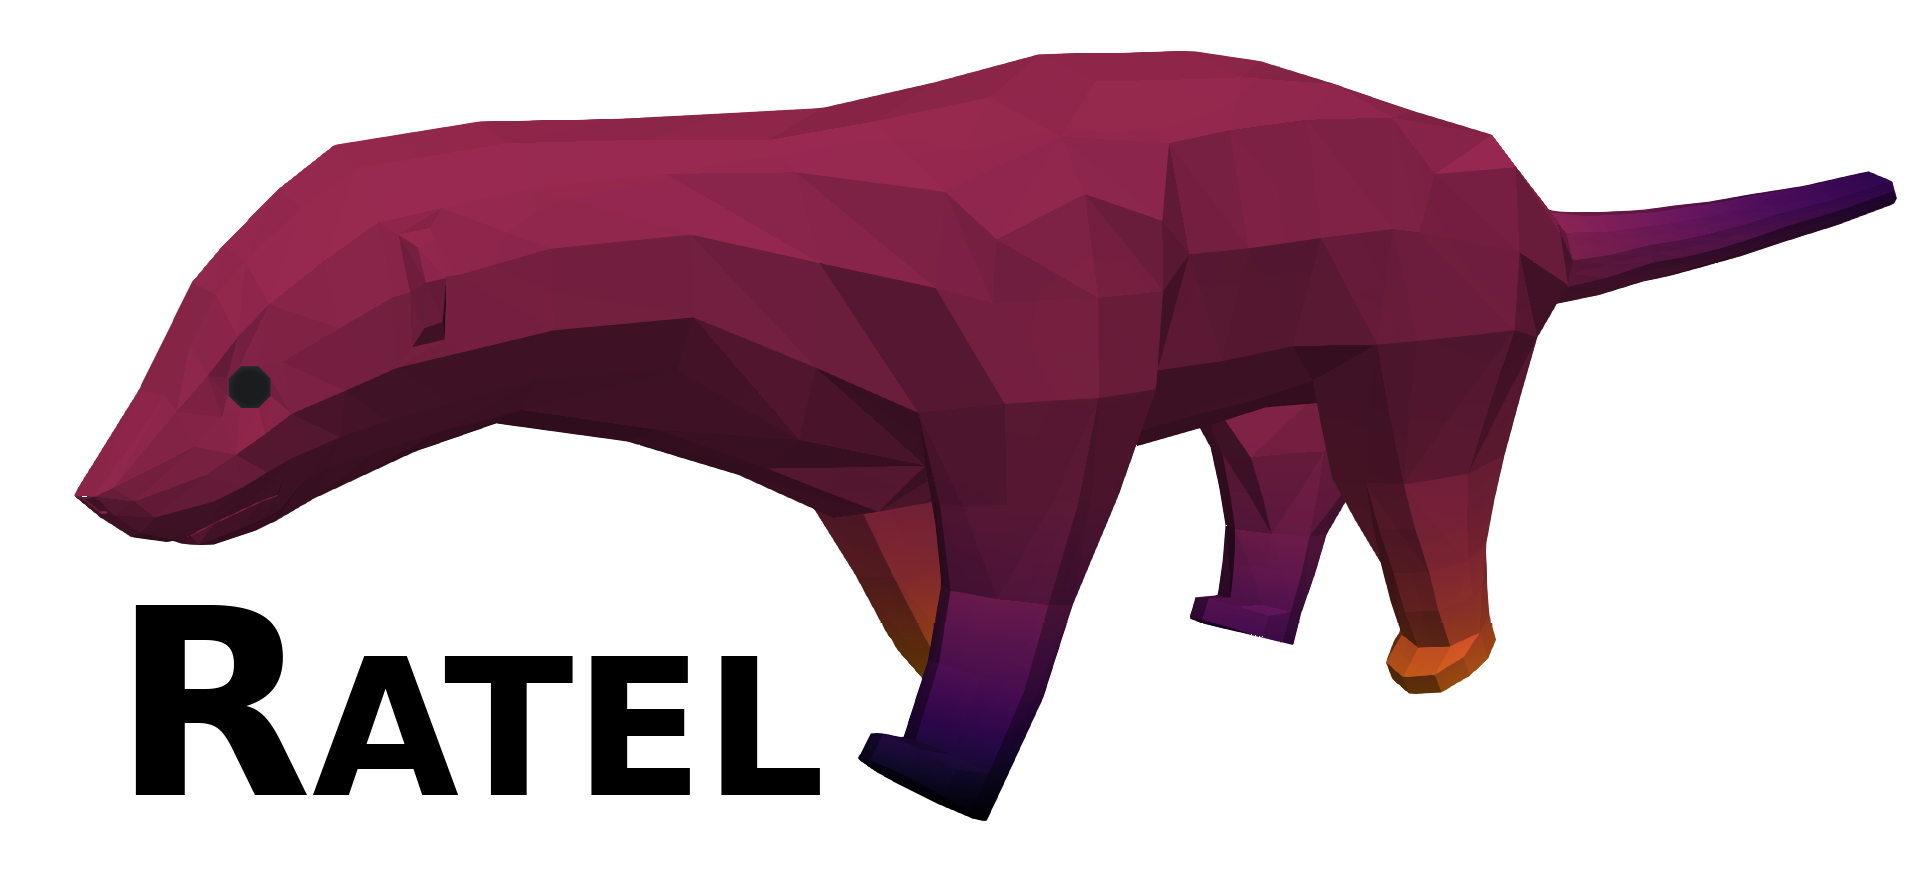
\includegraphics[width=\textwidth]{img/ratel-with-text.png}
            \includesvg[width=\textwidth]{img/libCEED.svg}
            \includesvg[width=\textwidth]{img/PETSc-TAO_RGB.svg}\\
        \end{center}
    \end{column}
    \begin{column}{0.6\textwidth}
        \begin{itemize}
            \item Implemented in Ratel, our matrix-free solid mechanics code built on libCEED and PETSc
            \item GPU: ROCm/HIP 7.1.2 on AMD Radeon VII (\texttt{\small gfx906:sramecc+:xnack-}, \~MI50) with \qty{16}{GB} HBM2 memory (CUDA also supported)
            \item CPU: AMD Ryzen 7 3700X, \qty{64}{GB} DDR4 RAM
            \item Solvers:
            \begin{itemize}
                \item libCEED \texttt{/gpu/hip/gen} backend
                \item Newton's method with backtracking line search
                \item BiCGStab(2) linear solver with Jacobi preconditioning
            \end{itemize}
        \end{itemize}
    \end{column}
\end{columns}
\end{frame}

\begin{frame}{Test Problem}
    \begin{columns}
        \begin{column}{0.5\textwidth}
            \centering
            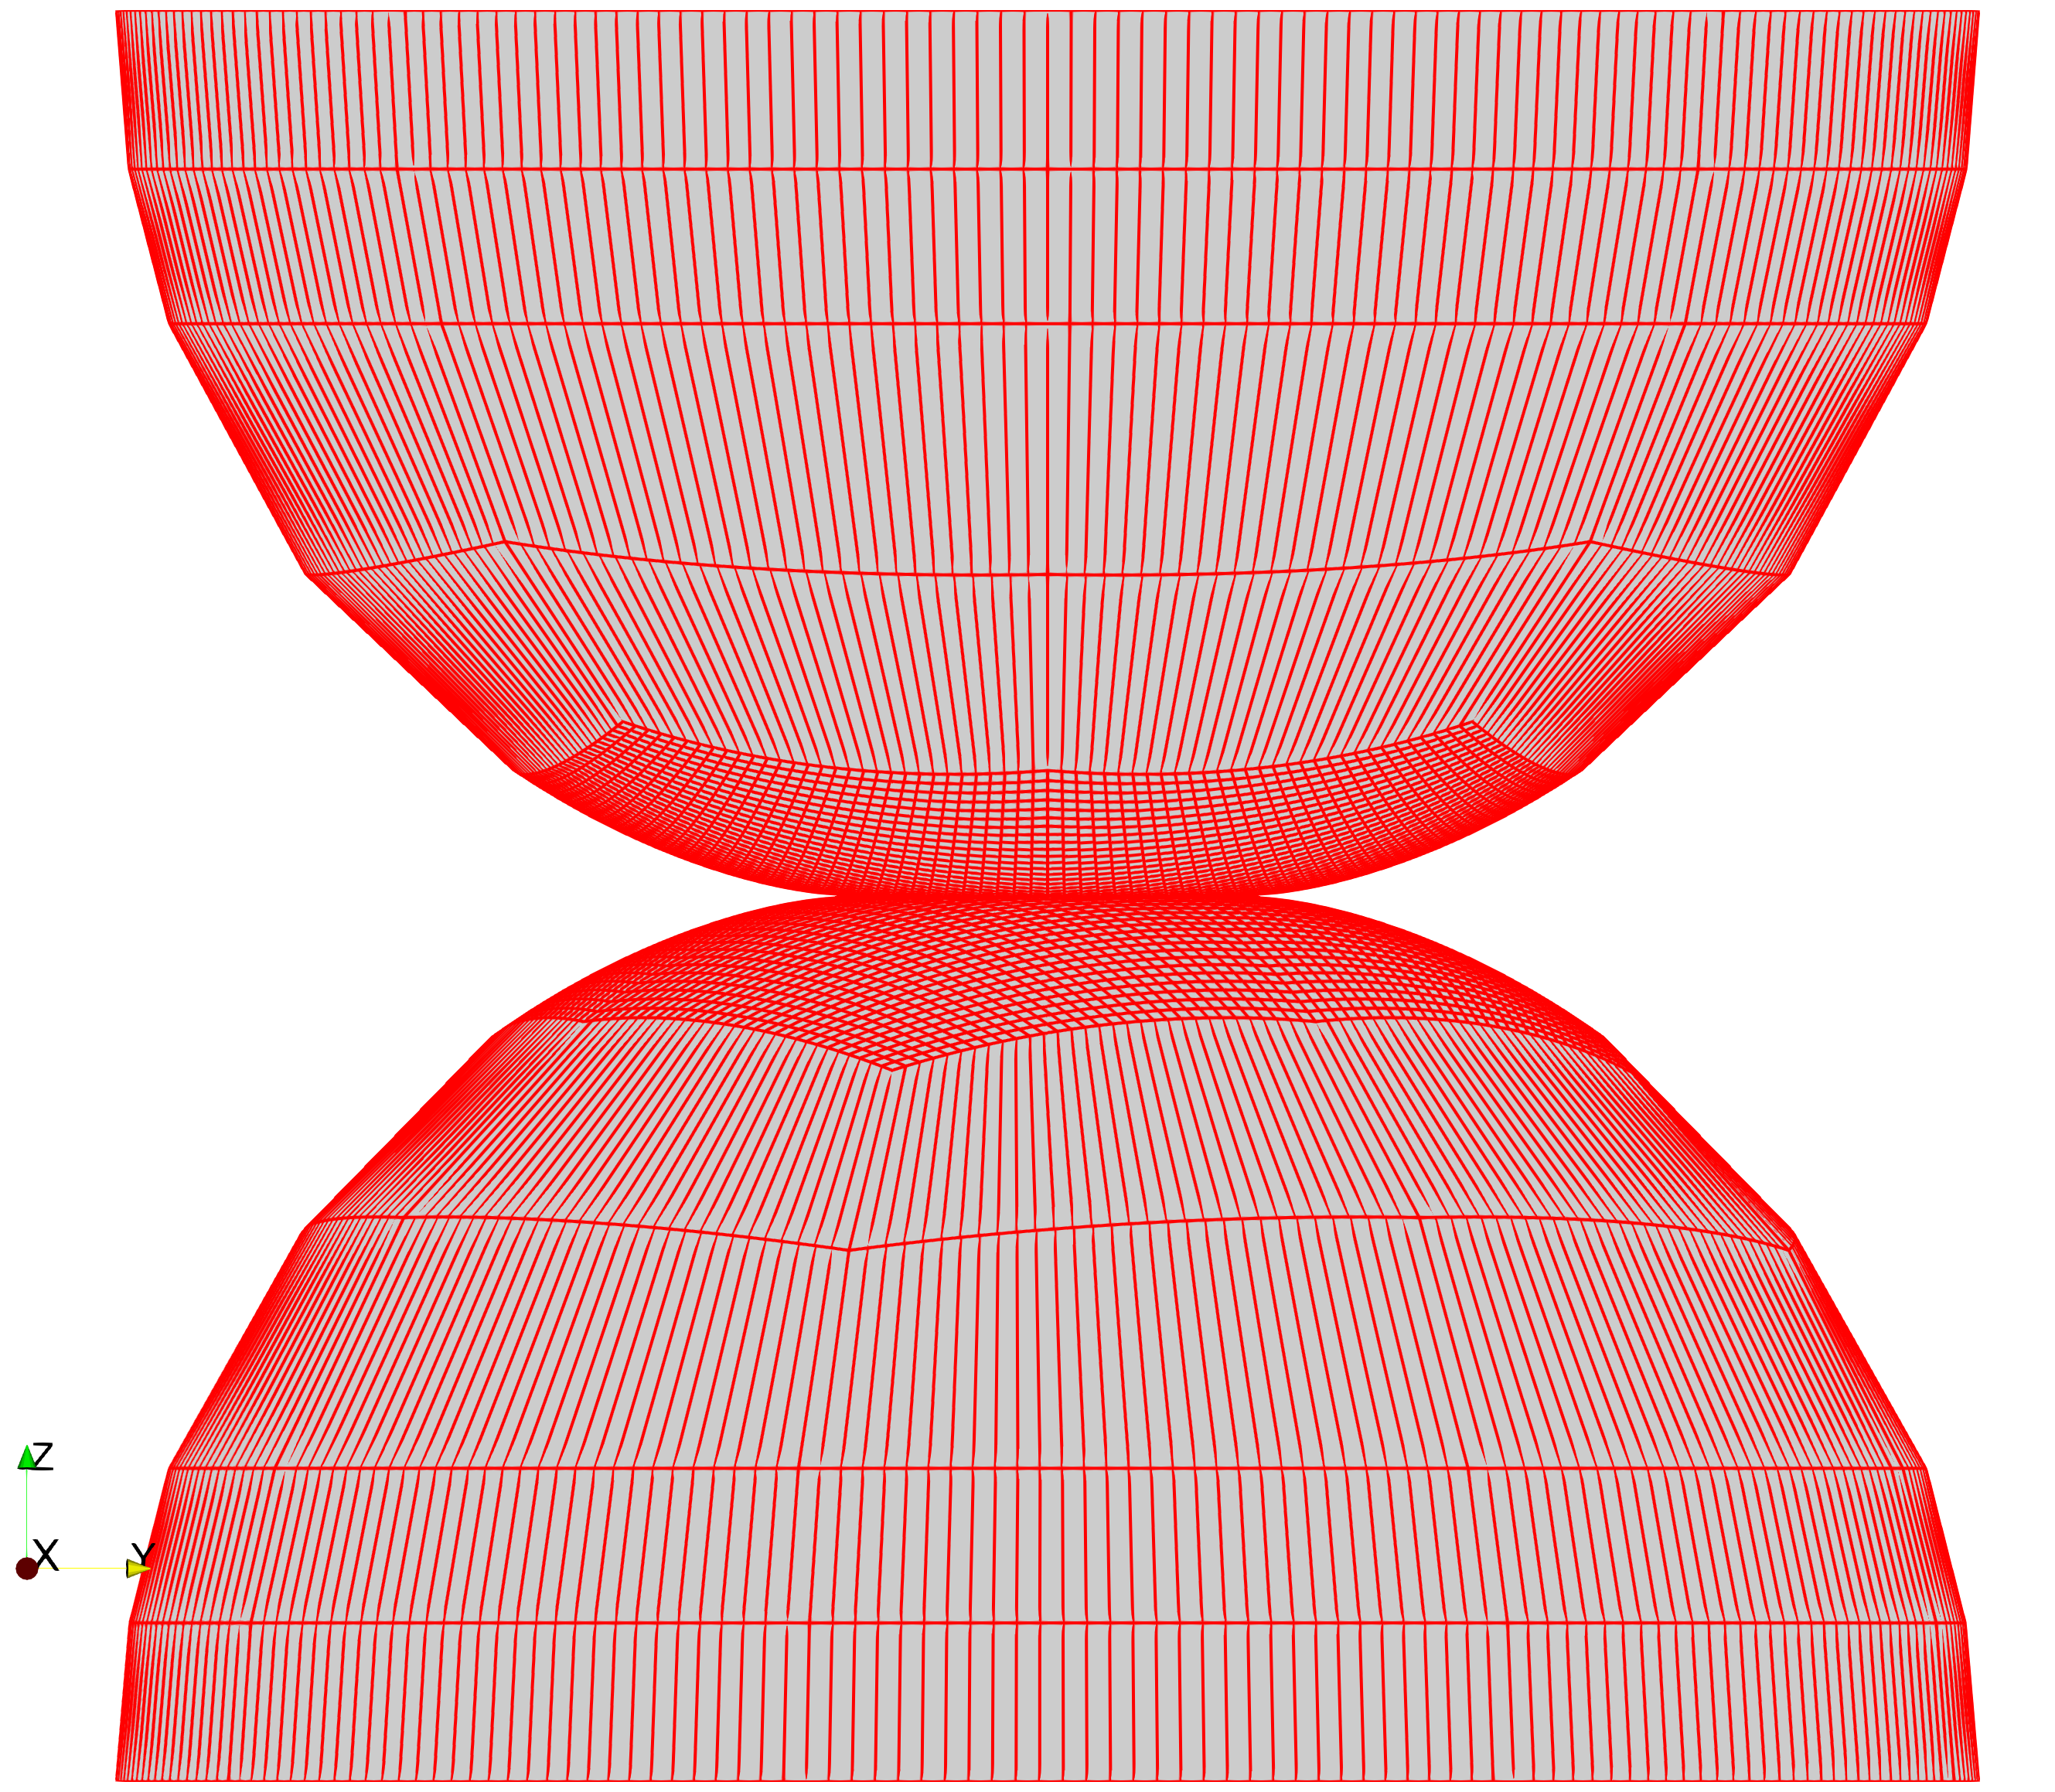
\includegraphics[height=\textheightwithtitle]{img/contact-problem-mesh.png}
        \end{column}
        \begin{column}{0.5\textwidth}
            \begin{itemize}
                \item Two half-spheres of radius $1$ in contact, displacement of $0.1$ on top surface
                \item Meshes are rotated \qty{30}{\degree} to increase clipping difficulty
                \item Only the area near contact surface is refined
                \begin{itemize}
                    \item Total DoFs between \num{1e4} and \num{2.4e6}
                    \item Total contact points between \num{2e3} and \num{1.1e6}
                \end{itemize}
                
            \end{itemize}
        \end{column}
    \end{columns}
\end{frame}

\begin{frame}{Wall Time}
    \begin{columns}
        \begin{column}{0.7\textwidth}
            \centering
            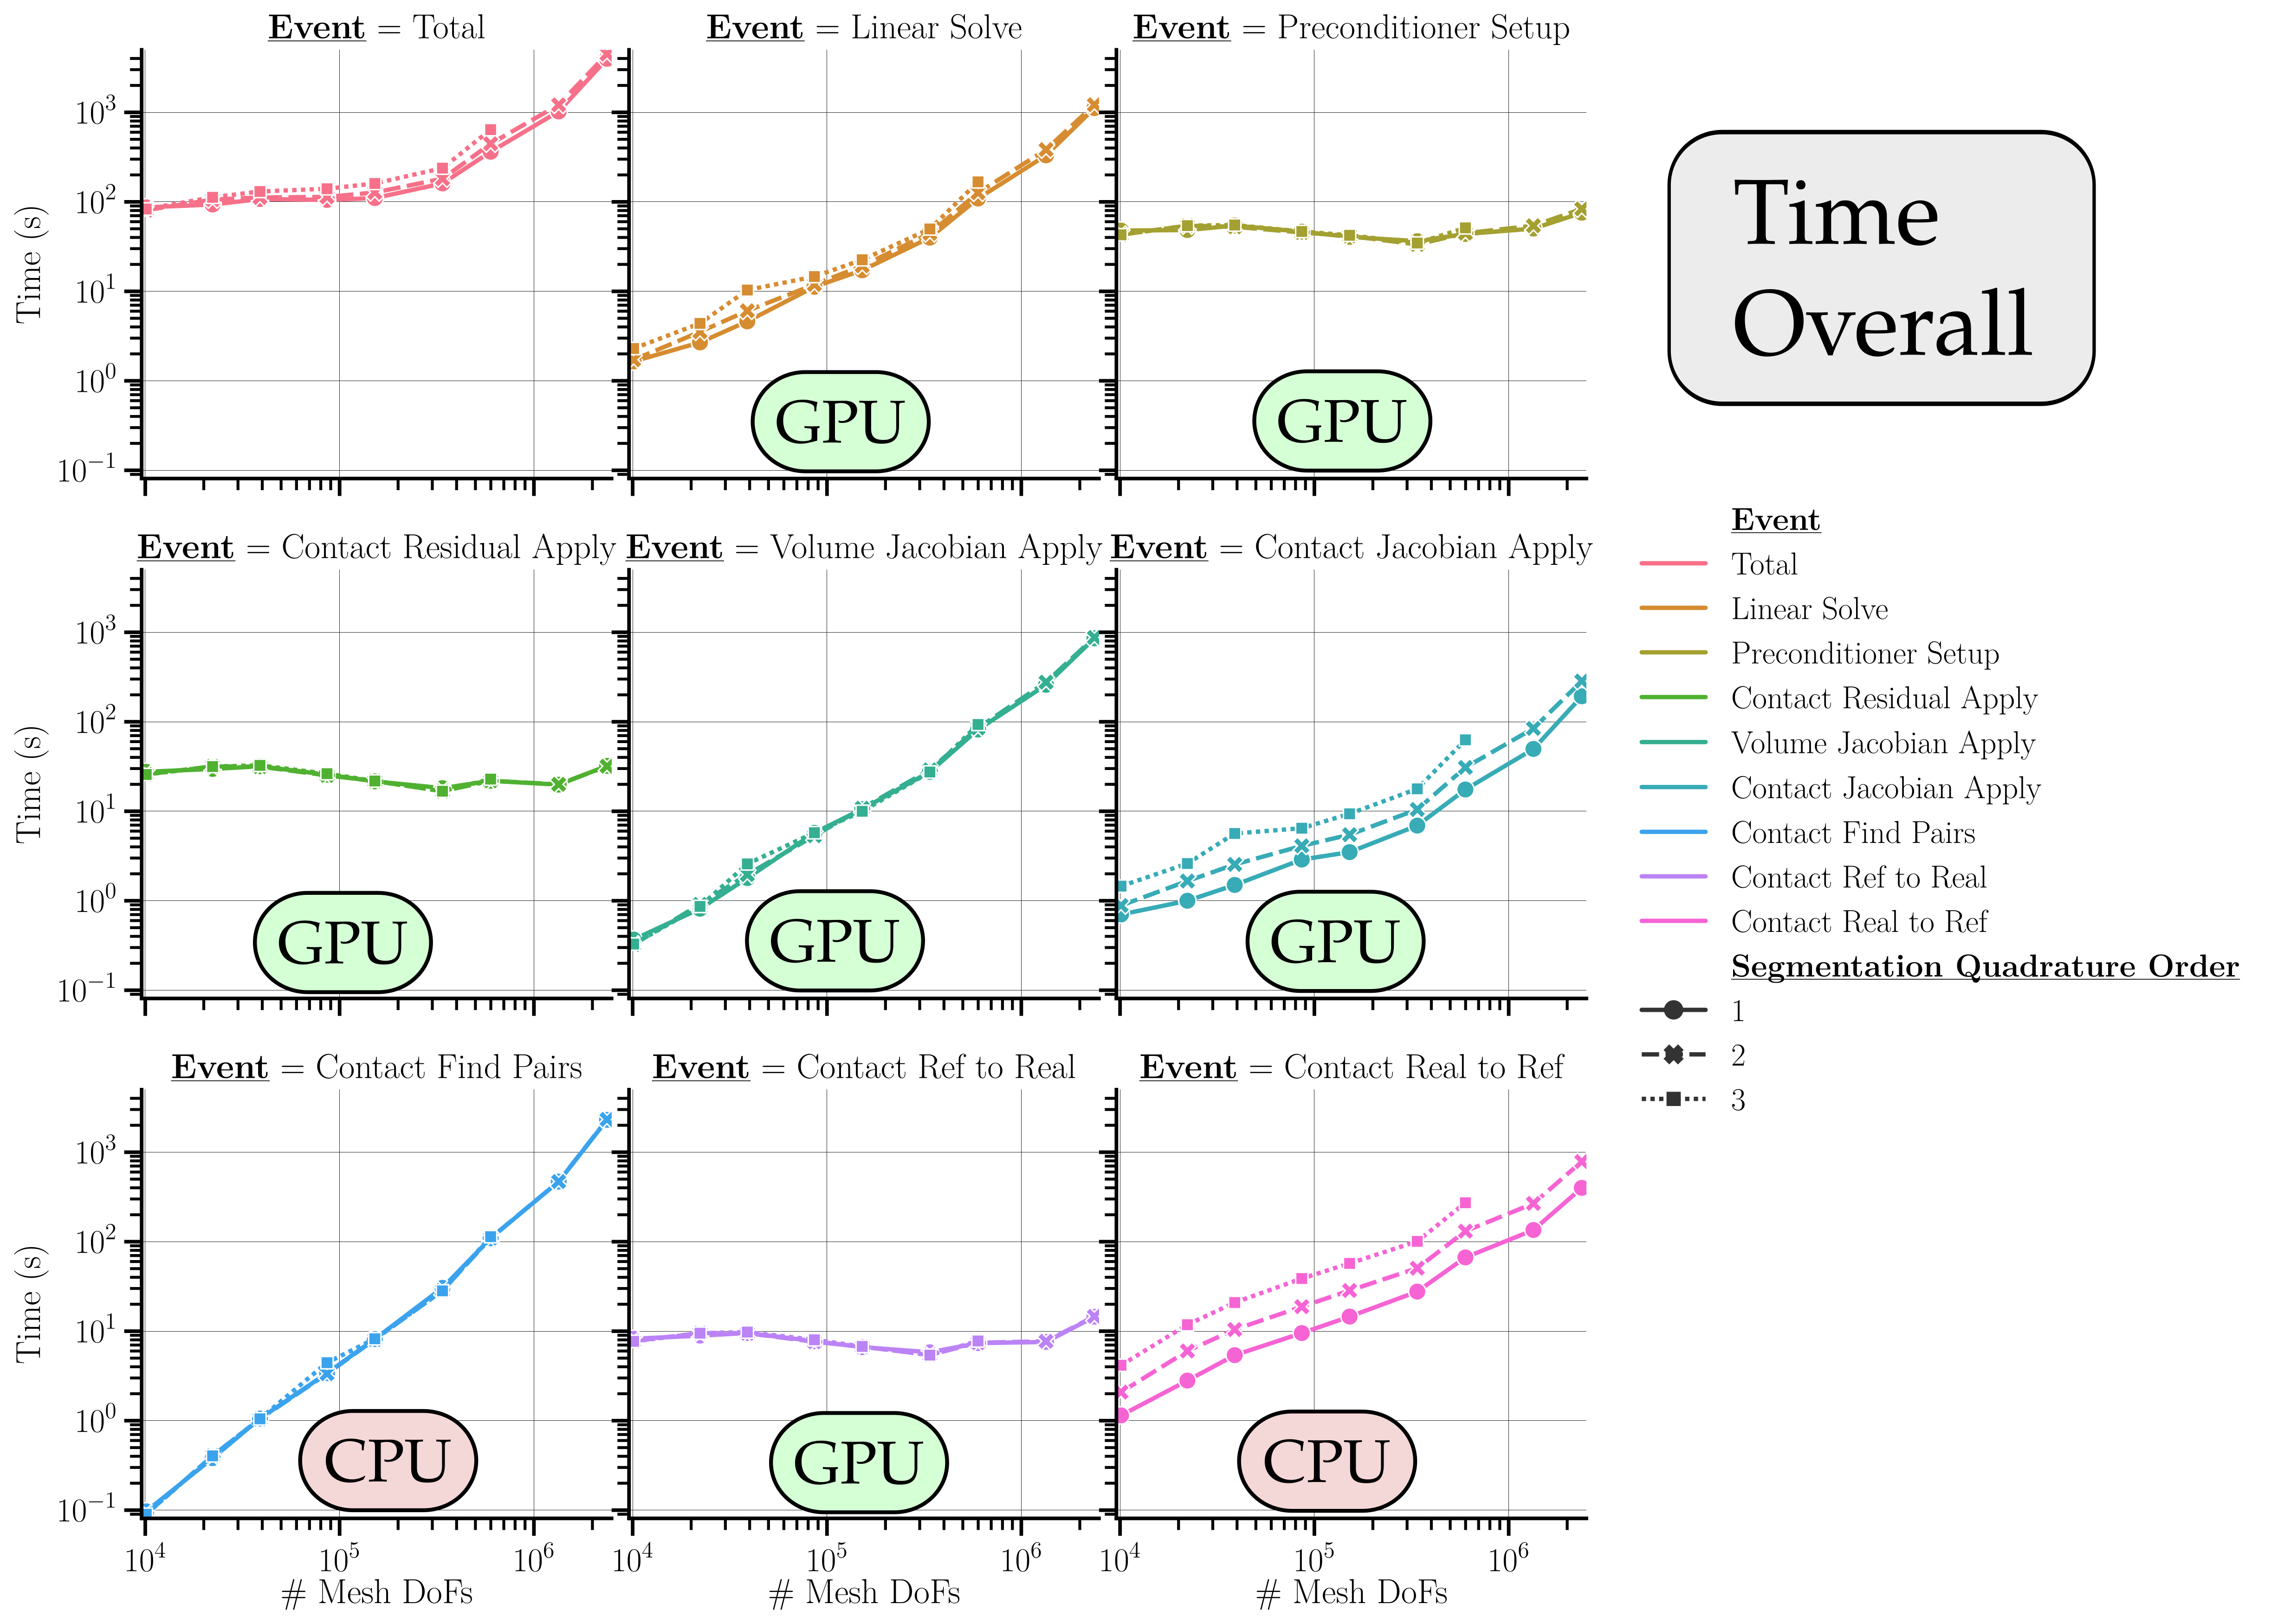
\includegraphics[height=\textheightwithtitle]{img/annotated_time_dofs.png}
        \end{column}
        \begin{column}{0.3\textwidth}
            \begin{itemize}
                \footnotesize
                \item All log-log, same scale
                \item Overall wall time --- slightly misleading due to more linear solver iterations at larger problem sizes (Jacobi preconditioning)
                \item Excluding CPU bound kernels, highest costs are diagonal assembly and (extremely efficient, see \cite{brown2022performanceportablesolidmechanics}) volume Jacobian application
            \end{itemize}
        \end{column}
    \end{columns}
\end{frame}

\begin{frame}{Efficiency}
    \begin{columns}
        \begin{column}{0.7\textwidth}
            \centering
            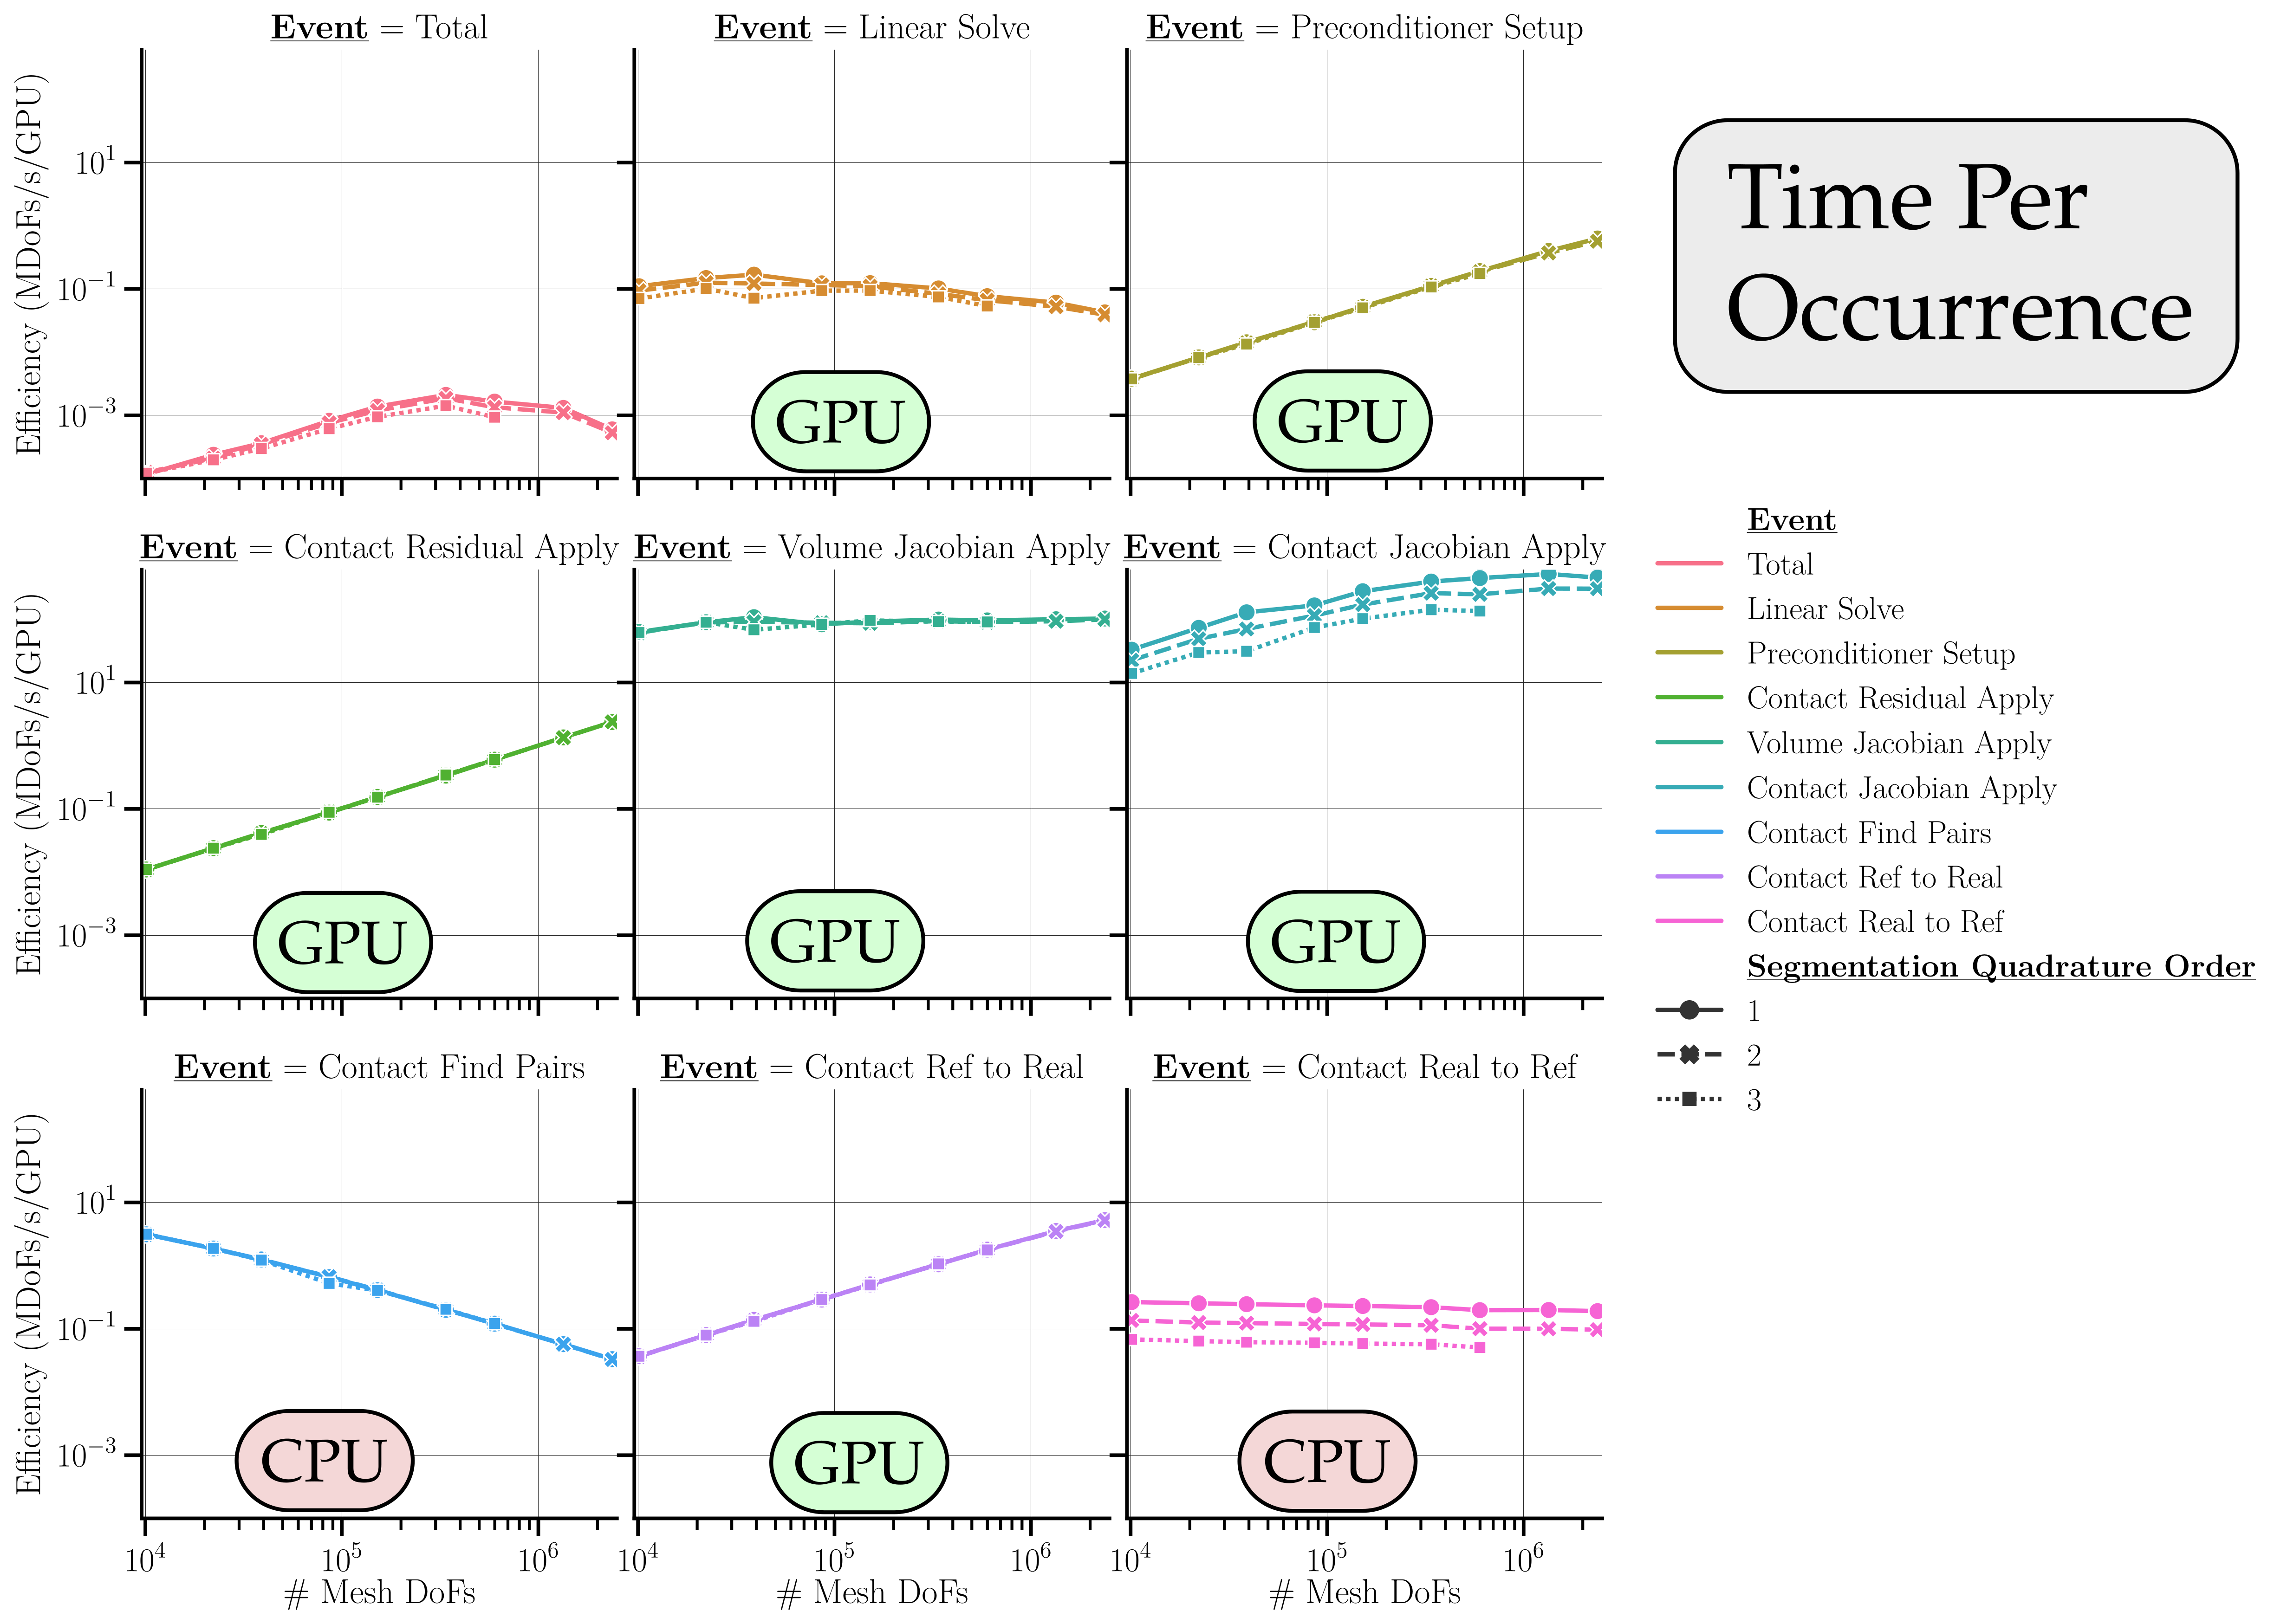
\includegraphics[height=\textheightwithtitle]{img/annotated_efficiency_dofs.png}
        \end{column}
        \begin{column}{0.3\textwidth}
            \begin{itemize}
                \footnotesize
                \item Higher is better
                \item All log-log, same scale
                \item Positive slope means larger problems use less time relative to problem size ($t \in \omega(\# \text{DoFs})$)
                \item Negative slope means time grows super-linear with DoFs ($t\in o(\# \text{DoFs})$)
                \item Primary bottleneck is all-to-all contact pair search --- not the focus of this talk
            \end{itemize}
        \end{column}
    \end{columns}
\end{frame}

\begin{frame}{Conclusions}
\begin{columns}
    \begin{column}{0.5\textwidth}
        \centering
        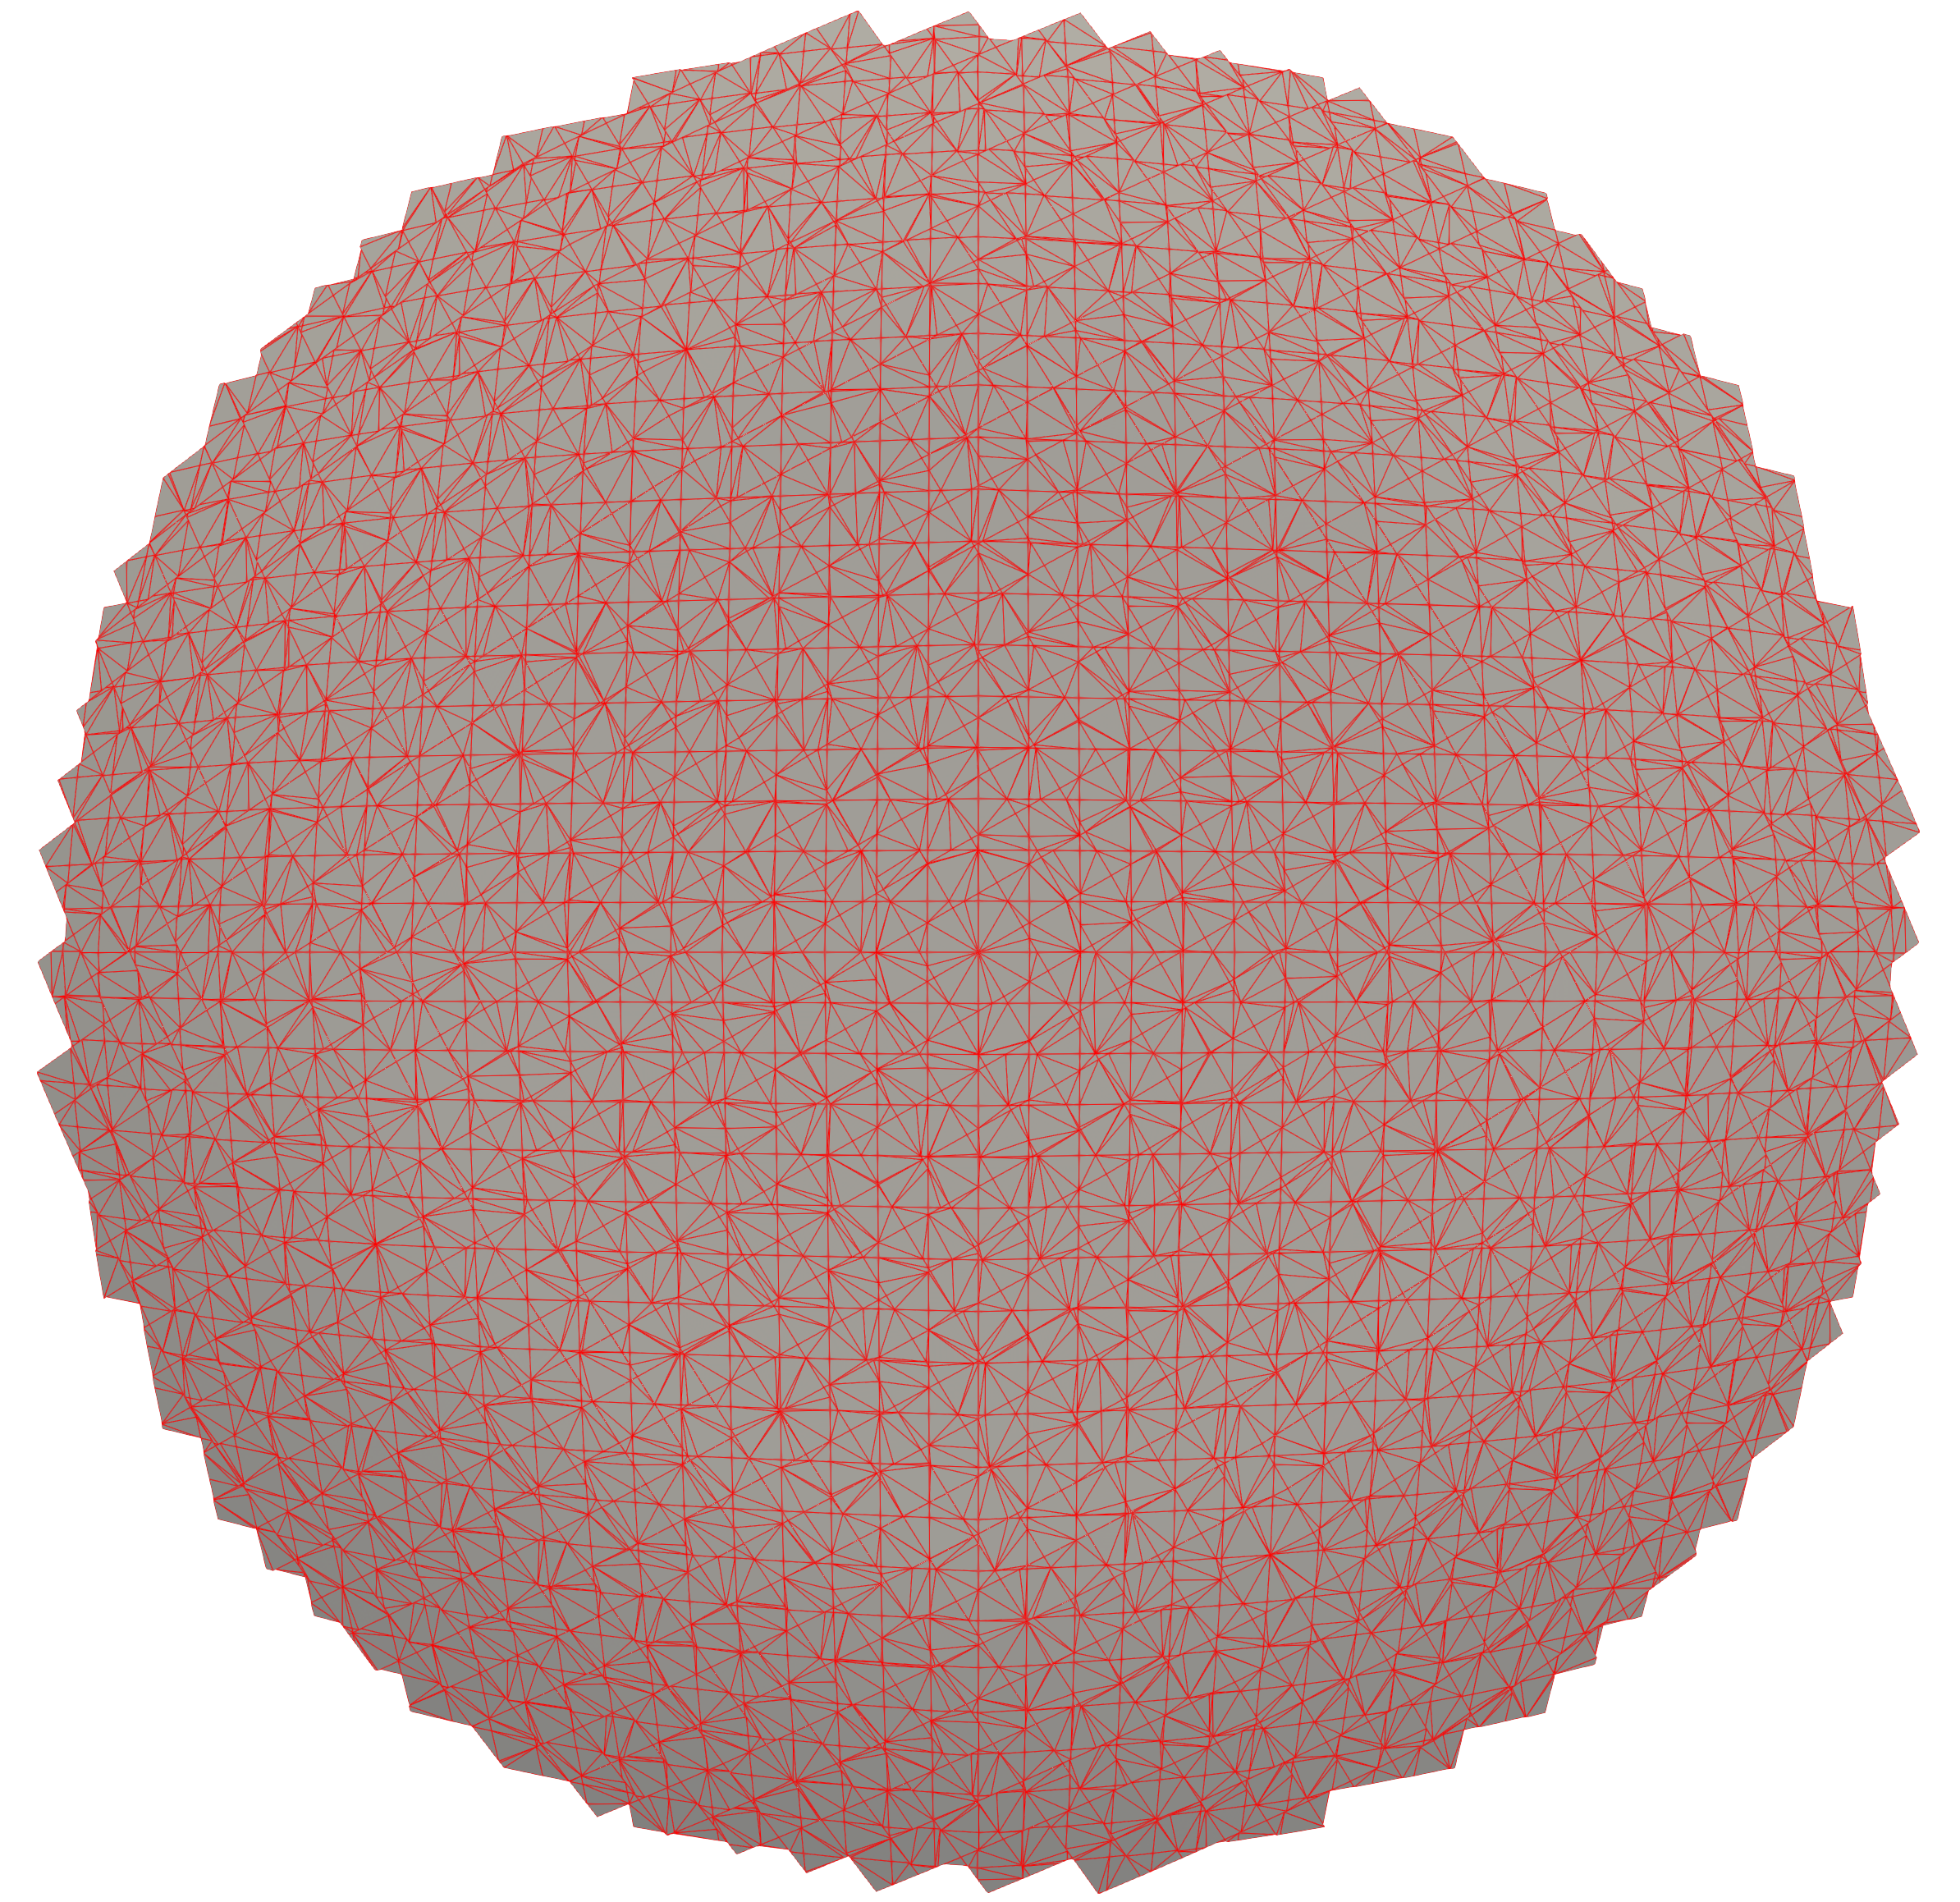
\includegraphics[height=\textheightwithtitle]{img/segmented-mesh.png}
        % 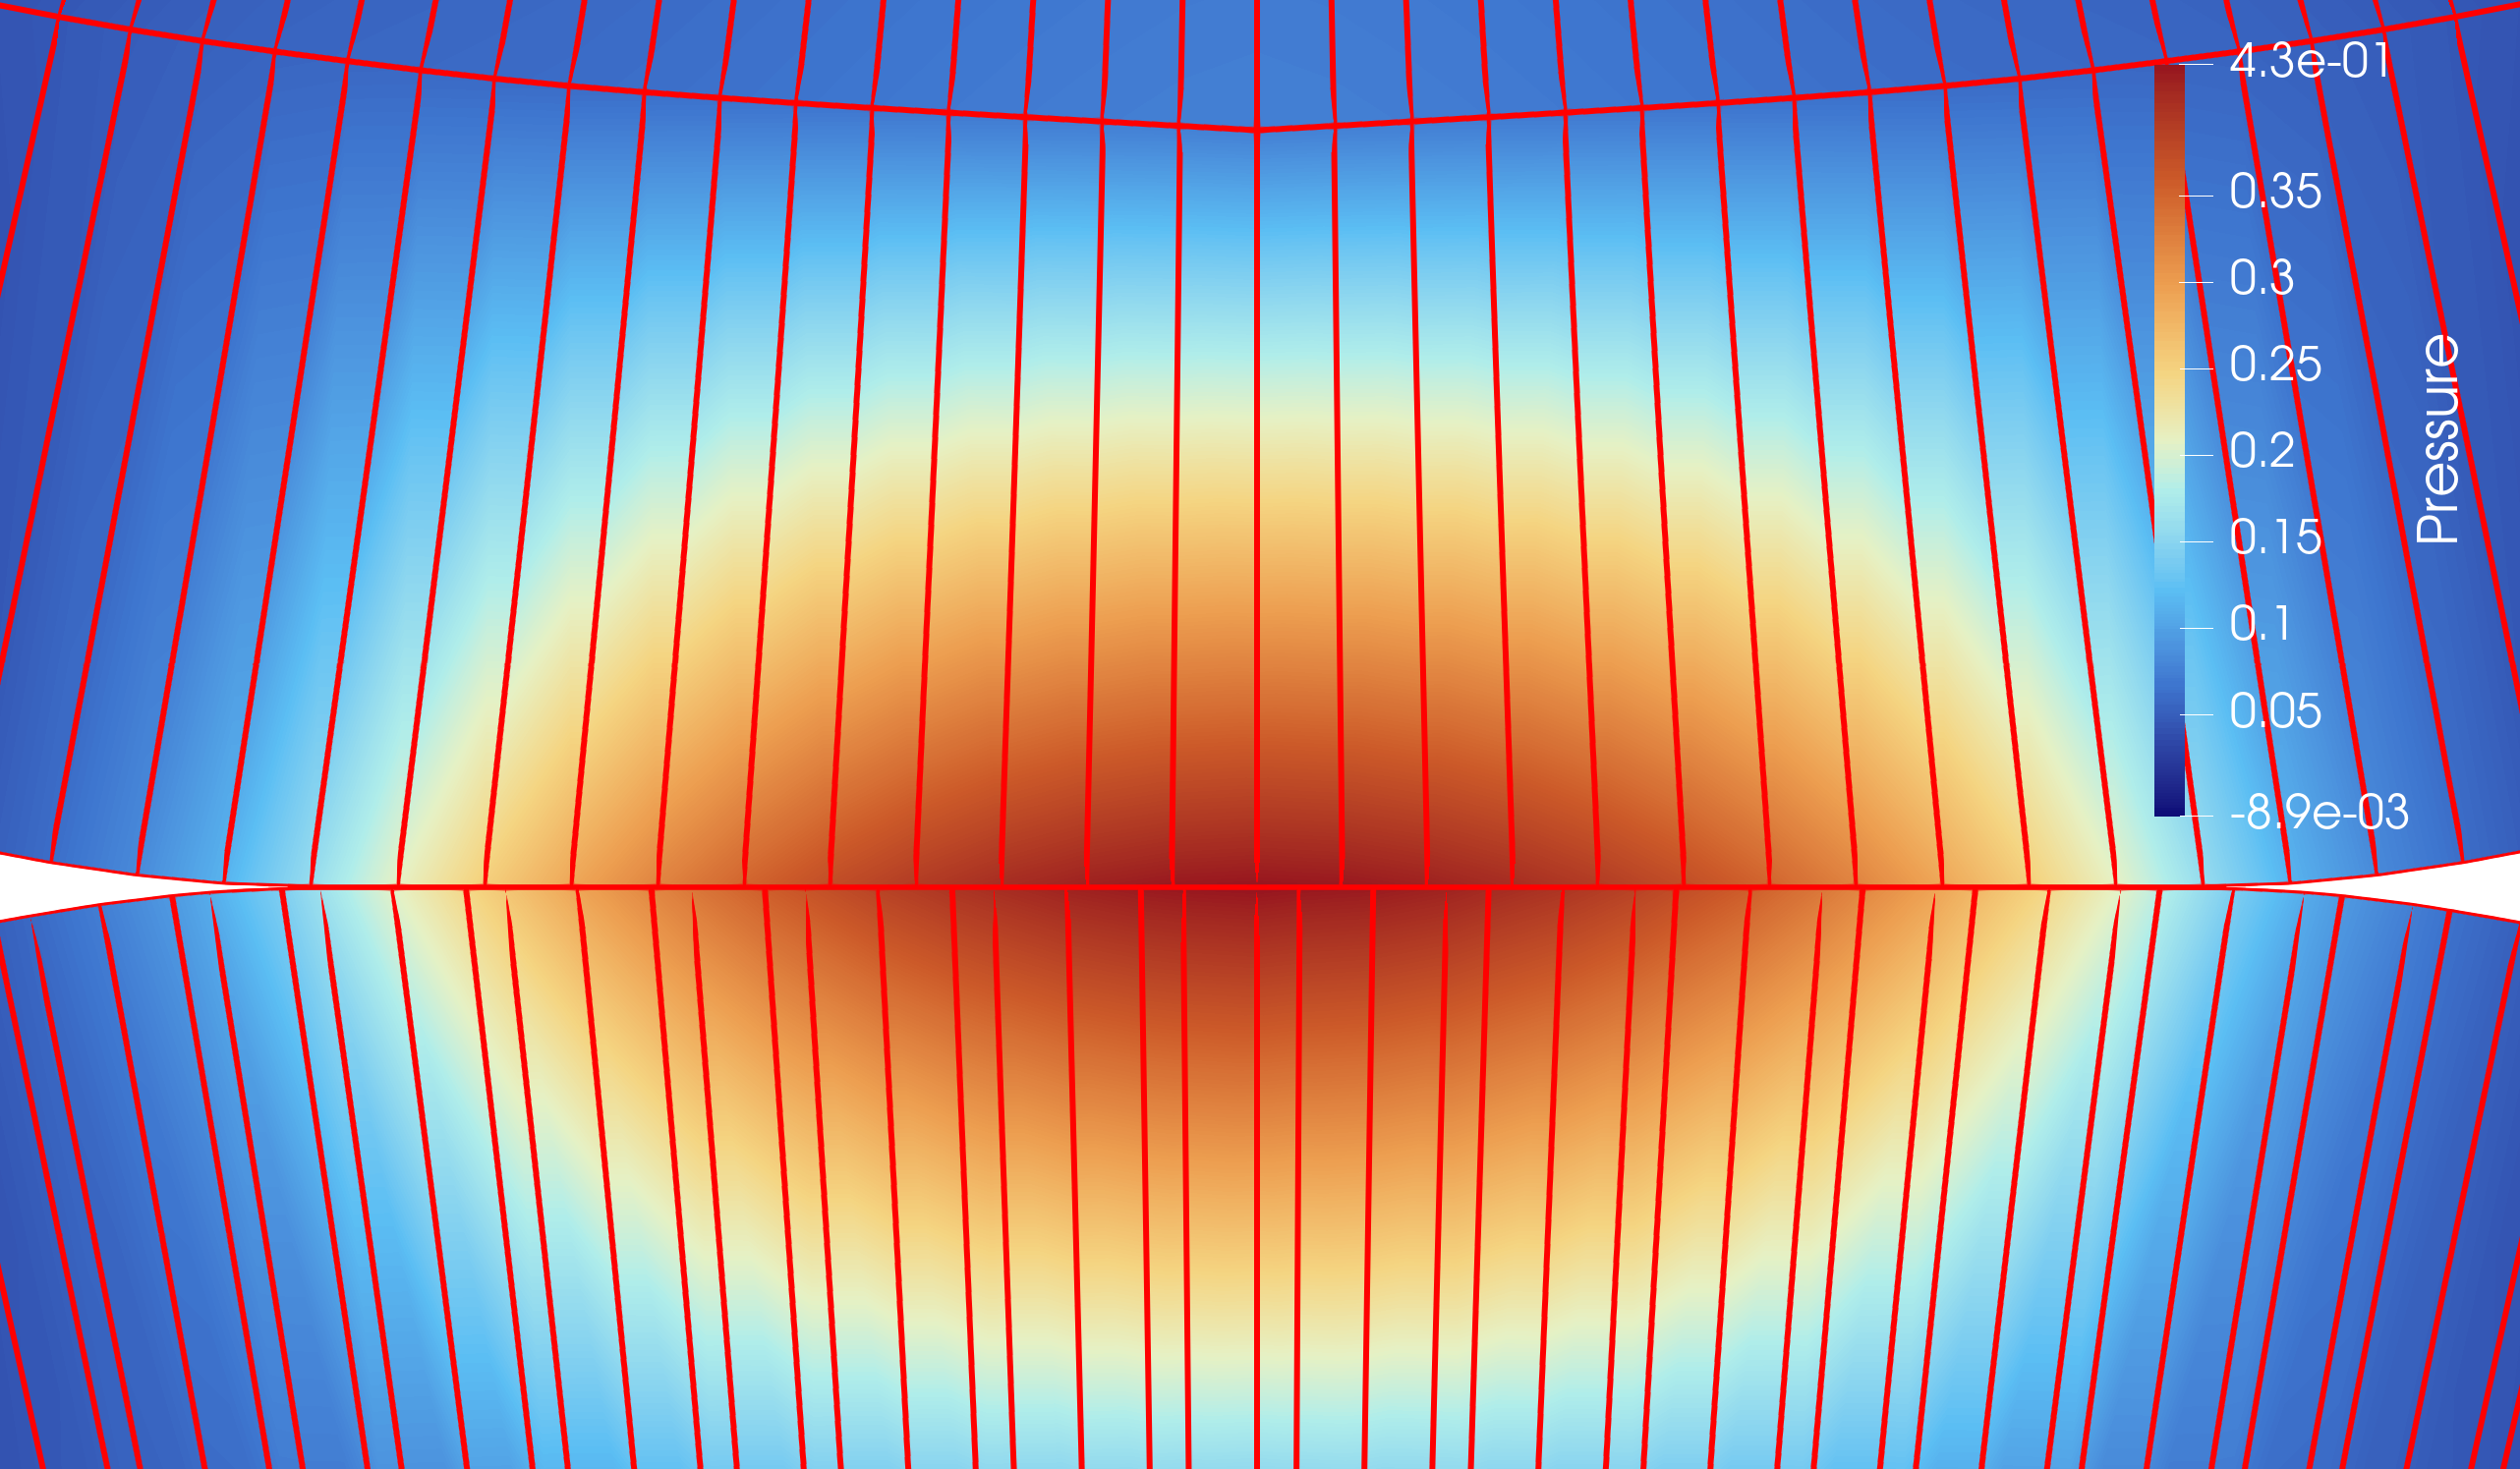
\includegraphics[width=0.7\textwidth]{img/contact-problem-pressure.png}
    \end{column}
    \begin{column}{0.5\textwidth}
    \begin{itemize}
        \item libCEED at-points matrix-free operators provide excellent performance for evaluating contact constraints across non-conforming boundaries
        \begin{itemize}
            \item Efficiency improves as problem sizes increase
        \end{itemize}
        \item Future work:
        \begin{itemize}
            \item Parallel/$O(n\log n)$ contact pair search
            \item Lagrange multipliers for contact forces \& field-split preconditioning 
            \item GPU offloading of contact pair evaluation and real-to-ref projections
        \end{itemize}
    \end{itemize}
    \end{column}
\end{columns}
    
\end{frame}




\begin{frame}[allowframebreaks]
    \printbibliography
\end{frame}

% Q&A
\begin{frame}[standout]
    \Huge\textsc{Thank You}
    
    \vfill
    
    \LARGE\textsc{Questions?}
\end{frame}

\appendix

\begin{frame}[c]{Aside: Similar Methods \& Future Applications}
\begin{twocolimgleft}{img/gfem.svg}
    \begin{exampleblock}{Generalized FEM (GFEM)}
        \begin{overlayarea}{\textwidth}{5\baselineskip}
            GFEM methods (\cite{Fries_Belytschko_2010}) also use cut elements, and the parallelization strategy described later could be applied for them as well
        \end{overlayarea}
    \end{exampleblock}
\end{twocolimgleft}
\end{frame}

\begin{frame}{Flame Graphs: $32^2$, $64^2$, \& $128^2$ Face Elements}
    \centering
    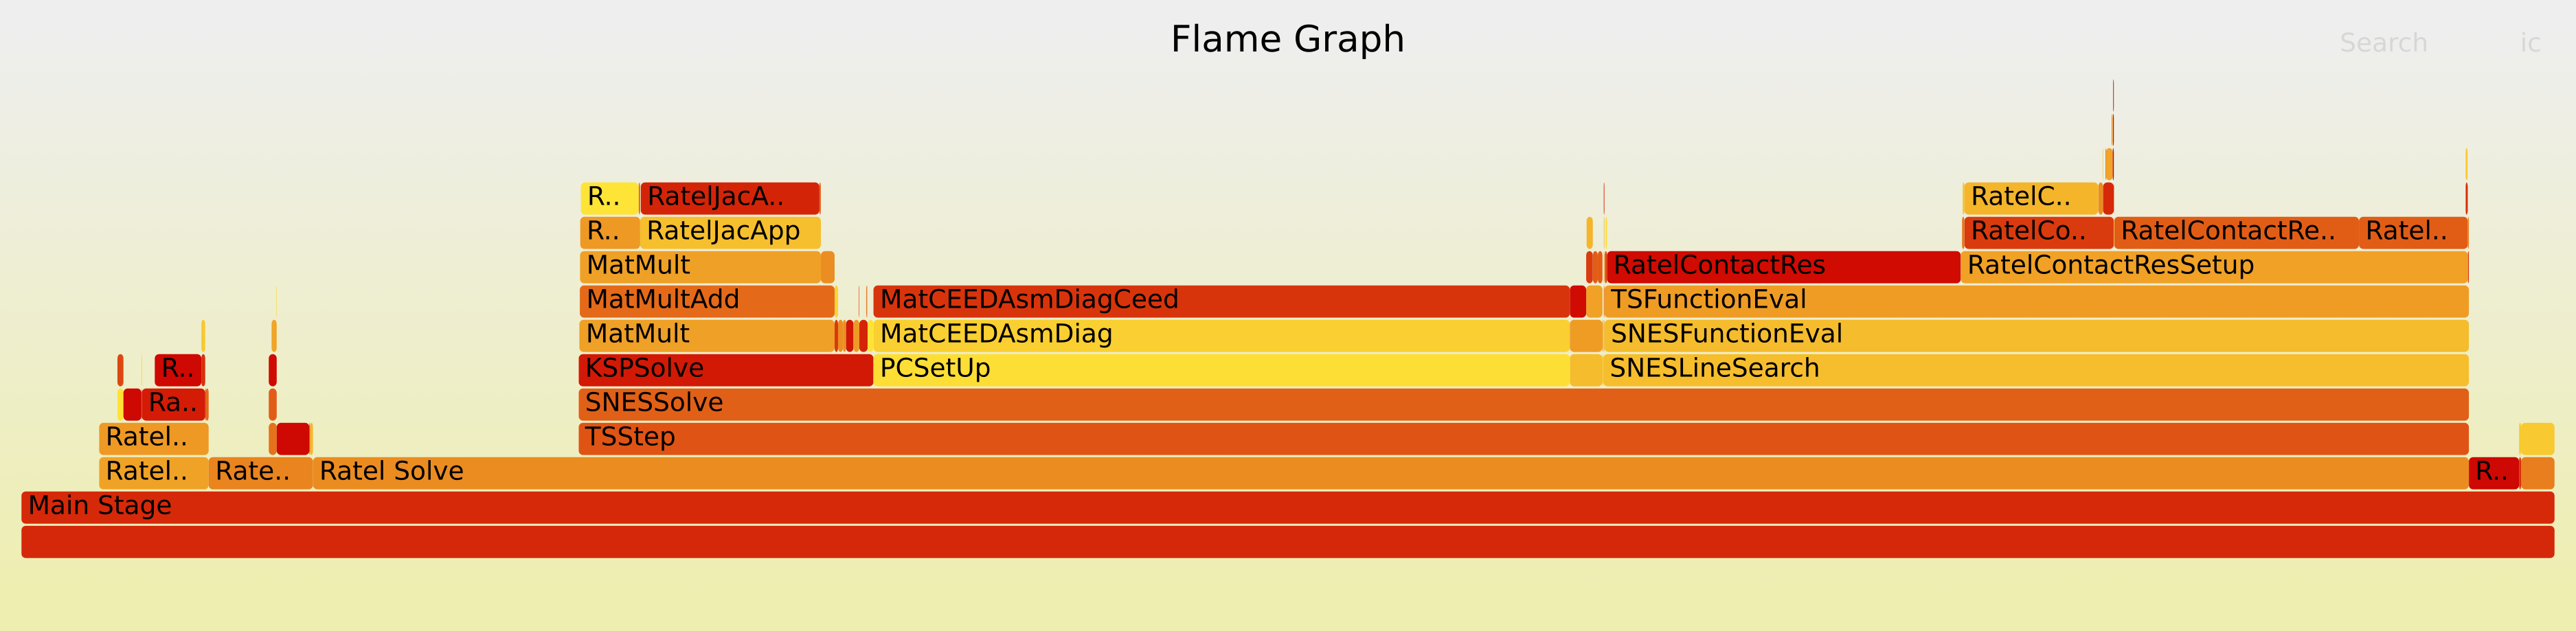
\includegraphics[height=0.33\textheightwithtitle]{img/ref_32_qextra_0}
    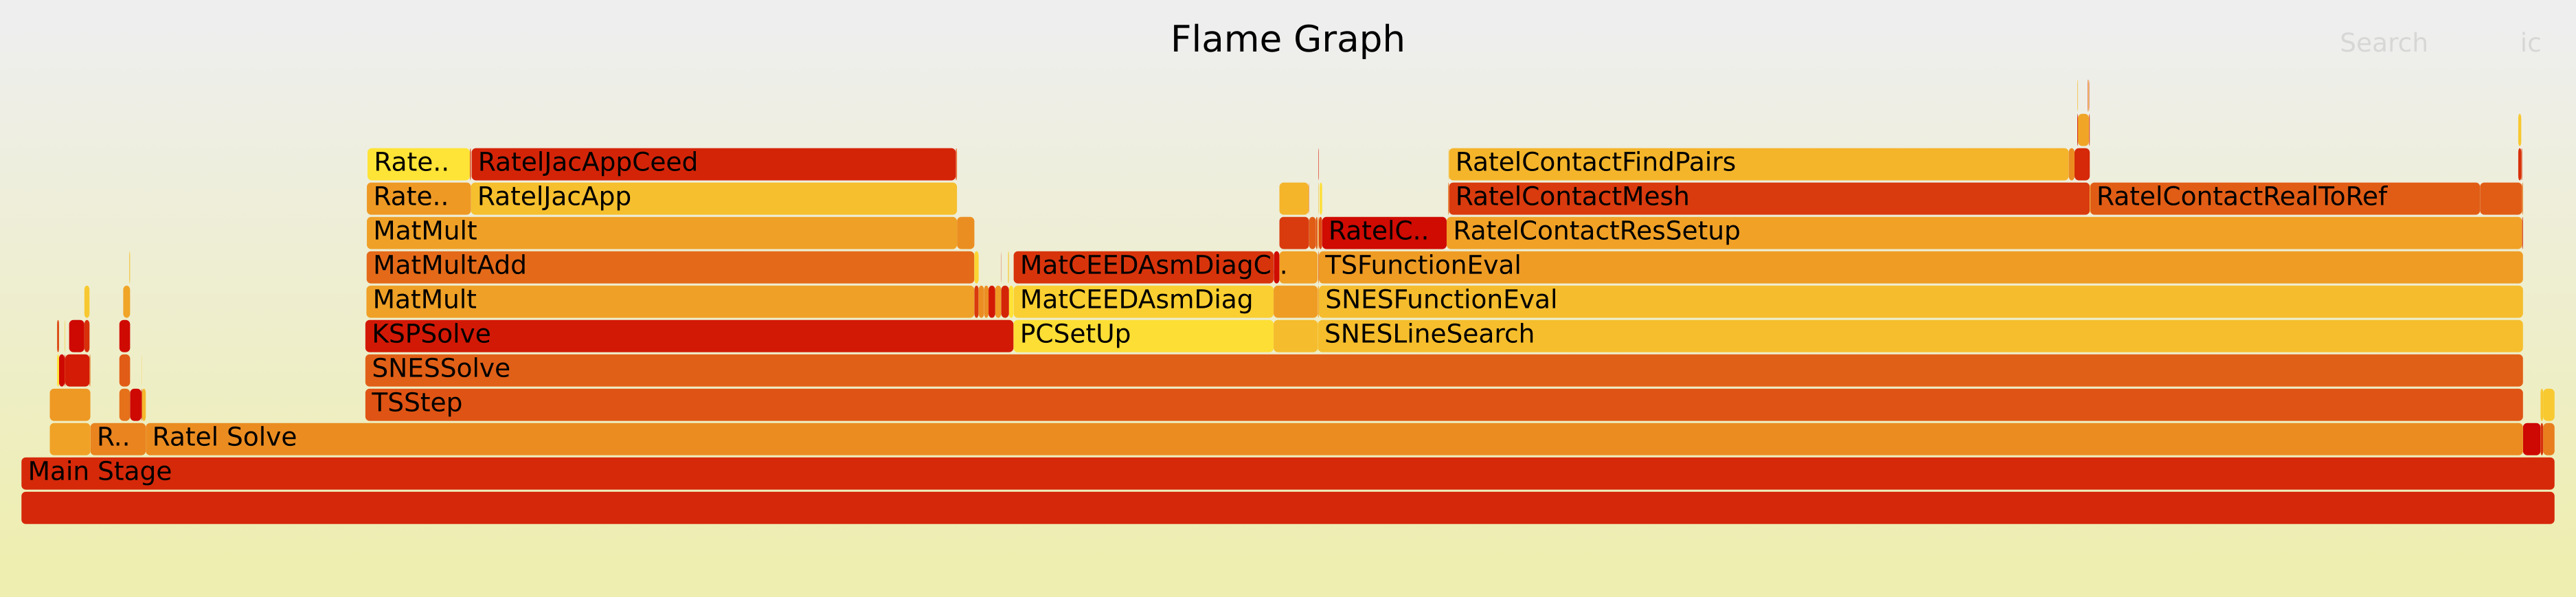
\includegraphics[height=0.33\textheightwithtitle]{img/ref_64_qextra_0}
    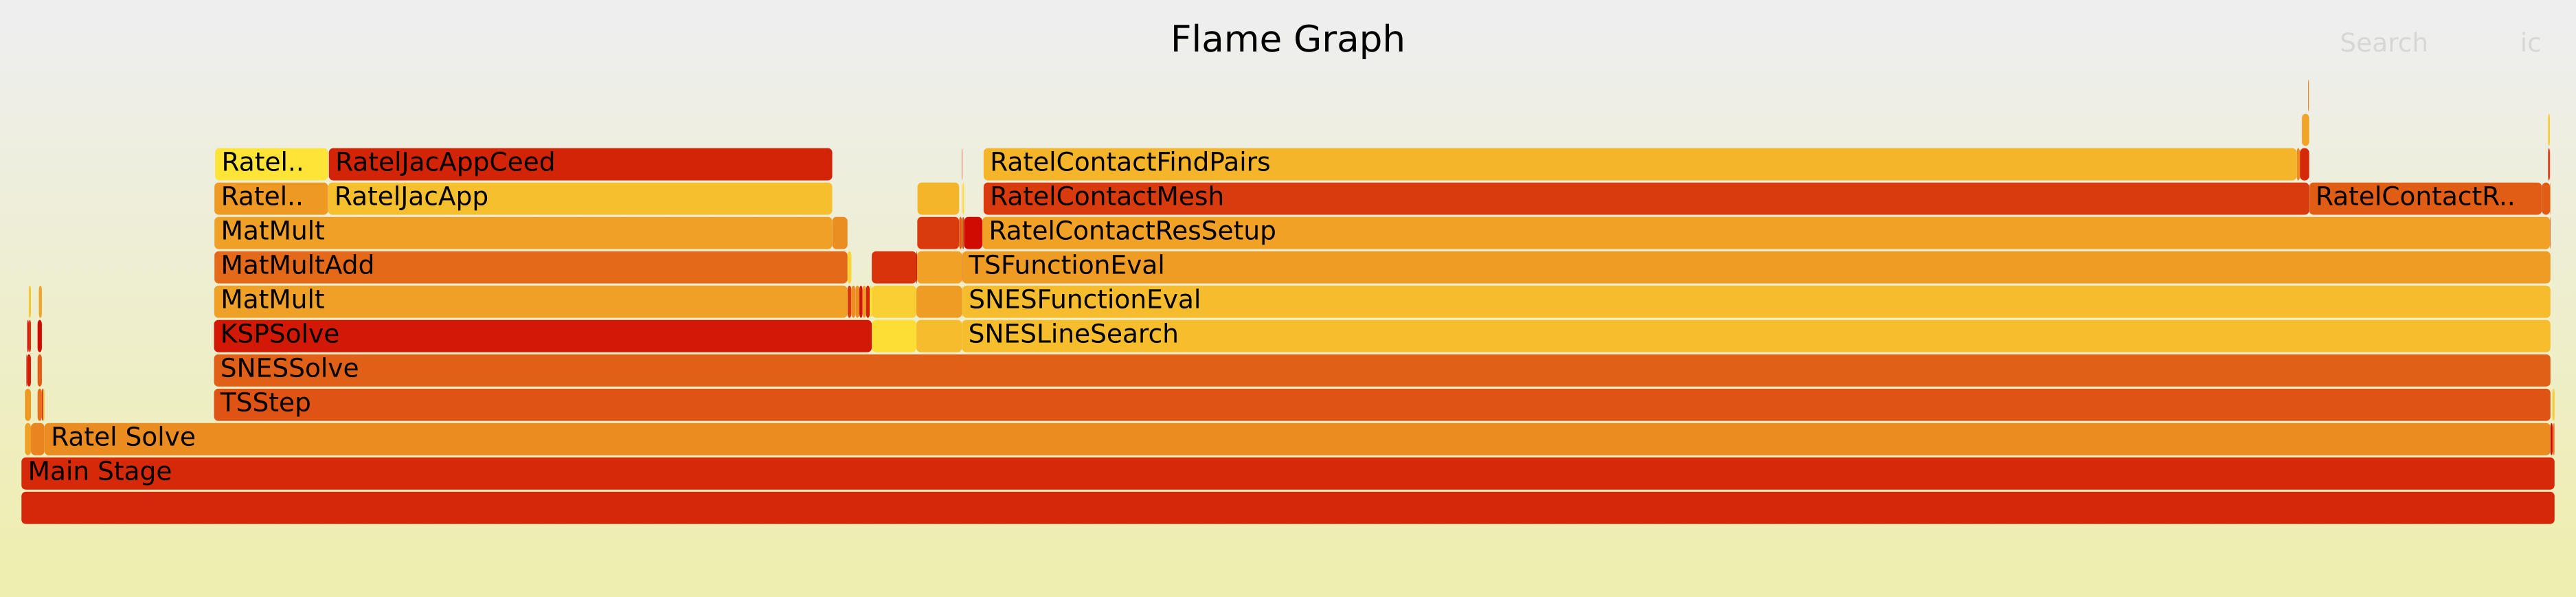
\includegraphics[height=0.33\textheightwithtitle]{img/ref_128_qextra_0}
\end{frame}

\begin{frame}{Rough Contact Operator Diagram}
    \centering
    \includesvg[height=\textheightwithtitle]{img/contact-operator-rough}
\end{frame}

\begin{frame}{Full Details on Basis Applications}
    \begin{align*} \sum _e \mathcal {E}^T \left[ \left( \mathbf{C} \mathbf{N} \right) ^T \mathbf{W}_p^e \Lambda \left( g_0 \left( u_p^e, \nabla u_p^e \right) \right) \right] \end{align*}
    with $u_p^e = \mathbf{N}_p^e \mathbf{C} \mathbf{N} \mathcal {E}^e u$, $\nabla u_p^e = \lbrace \mathbf{D}_{p, i}^e \mathbf{C} \mathbf{N} \mathcal {E}^e u \rbrace _{i = 0}^{d - 1}$, $\mathbf{C} \mathbf{N} = (CN) \otimes (CN) \otimes (CN)$ and
    \begin{align*}
        \mathbf{N}_p^e &= N^e_{p,0} \otimes N^e_{p,1},\\ \mathbf{D}_{p,0}^e = D^e_{p,0} \otimes N^e_{p,1},&\quad
        \mathbf{D}_{p,1}^e = N^e_{p,0} \otimes D^e_{p,1} \\
        (N^e_{p,d})_{ij} &= T_j\del{(\bm \xi^e_i)_d}, \quad d = 0,1\\
        (D^e_{p,d})_{ij} &= \frac{\dif T_j}{\dif \xi}\del{(\bm \xi^e_i)_d}, \quad d = 0,1\\
    \end{align*}
\end{frame}
    
\begin{frame}{Computing the Integral Over the Surface}
\begin{twocolimgleftratio}{img/segmentation_multi_back_to_nonmortar.svg}{0.5}
    \centering
    \includesvg[height=0.9\textheightwithtitle,width=\linewidth]{img/segmentation_multi_equation}
\end{twocolimgleftratio}
\end{frame}

\end{document}
